%% FEUP THESIS STYLE
%% originally by JCL & JCF, modified by nhopf

%% One-sided output by default
\documentclass[11pt,a4paper]{report}
%% For two-sided printing (for dead-tree output) comment previous line and uncomment the next line
%\documentclass[11pt,a4paper,twoside,openright]{report}

\usepackage[utf8]{inputenc}
\usepackage{notoccite}
\usepackage{multirow} % Include this for \multirow command

%% Thesis style
\usepackage{feupteses}
%% Additional options for feupteses.sty:
%% - onpaper: links are not shown (for paper versions)
%% - backrefs: include back references from bibliography to citation  place

%% Uncomment the next lines if side by side graphics used
\usepackage[lofdepth,lotdepth]{subfig}
\usepackage{float}
\usepackage{longtable}
\usepackage{lipsum}
\usepackage{enumitem}
\usepackage{subcaption}  % for subfigures


% Listings
\definecolor{cloudwhite}{cmyk}{0,0,0,0.025}  % color

%% Include source-code listings package
\usepackage{listings}
\lstset{ %
    language=C,                        % choose the language of the code
    basicstyle=\footnotesize\ttfamily,
    keywordstyle=\bfseries,
    numbers=left,                      % where to put the line-numbers
    numberstyle=\scriptsize\texttt,    % the size of the fonts that are used for the line-numbers
    stepnumber=1,                      % the step between two line-numbers. If it's 1 each line will be numbered
    numbersep=8pt,                     % how far the line-numbers are from the code
    frame=tb,
    float=htb,
    aboveskip=8mm,
    belowskip=4mm,
    backgroundcolor=\color{cloudwhite},
    showspaces=false,                  % show spaces adding particular underscores
    showstringspaces=false,            % underline spaces within strings
    showtabs=false,                    % show tabs within strings adding particular underscores
    tabsize=2,                         % sets default tabsize to 2 spaces
    captionpos=b,                      % sets the caption-position to bottom
    breaklines=true,                   % sets automatic line breaking
    breakatwhitespace=false           % sets if automatic breaks should only happen at whitespace
}

%% Uncomment to create an index (at the end of the document)
%\makeindex

%% Path to the figures directory
\graphicspath{{figures/}}

%%----------------------------------------
% some macro definitions

% format
\newcommand{\class}[1]{{\normalfont\slshape #1\/}}

% entities
\newcommand{\Feup}{Faculdade de Engenharia da Universidade do Porto}

\newcommand{\svg}{\class{SVG}}
\newcommand{\scada}{\class{SCADA}}
\newcommand{\scadadms}{\class{SCADA/DMS}}

%%----------------------------------------

%%========================================
%% Start of document
%%========================================
\begin{document}

%%----------------------------------------
%% Information about the work
%%----------------------------------------
    \title{Vision-aided Open Radio Access Network}
    \author{Carolina Simões}

%% Uncomment next line for date of submission
    \thesisdate{Oct 16, 2024}

%% Comment next line copyright text if not used
    \copyrightnotice{Carolina Simões, 2024}

    \supervisor{Supervisor}{Prof. Manuel Ricardo}

%% Uncomment next line if necessary
    \supervisor{Second Supervisor}{Dr. André Coelho}

%% Uncomment committee stuff in the final version if used
%\committeetext{Approved by \ldots:}
%\committeemember{President}{Name of the President}
%\committeemember{Referee}{Name of the Referee}
%\committeemember{Referee}{Name of the Referee}
%\signature

%% Specify cover logo (in folder ``figures'')
    \logo{uporto-feup.pdf}

%% Uncomment next line for additional text below the author's name (front page)
%\additionalfronttext{Dissertation Planning}

%%----------------------------------------
%% Preliminary materials
%%----------------------------------------

% remove unnecessary \include{} commands
    \begin{Prolog}
        
\chapter*{Abstract}
%\addcontentsline{toc}{chapter}{Abstract}

This document introduces the preliminary work on a perception-aided solution for 6G networks, addressing the increasing demands of users and overcoming limitations posed by proprietary solutions. It provides insights into the paradigms and applications of 5G and 6G networks and deployment approaches for Radio Access Networks (RANs). The document explores computer vision detection and tracking models, highlighting relevant work on blockage prediction, proactive handover, and O-RAN. It also presents the Horizon Europe CONVERGE research project. The main objective of this dissertation is to implement vision-based functionality into a 6G Base Station (gNB), paving the way for obstacle-aware networks. Specific objectives include implementing object detection and tracking mechanisms, developing a Vision-Enabled gNB Enhancement Application for real-time perception, creating a web service for information dissemination, and researching validation in networking scenarios. The document presents a proposed solution and outlines a work plan for the dissertation, detailing objectives that involve integrating computer vision tools with a service-oriented network architecture to support the operation of a perception-aided Base Station. The proposed solution aims to enable obstacle-aware networks by providing video-based information to a 6G Base Station repositioning. To validate the solution's effectiveness, a use case illustrating the synergy between computer vision, machine learning, and wireless communications will be considered, to demonstrate the potential of visual perception for seamless wireless connectivity. % the abstract
        \cleardoublepage
        \chapter*{Resumo}
A evolução das redes móveis, caracterizada pelo aumento da complexidade e pela dependência de soluções proprietárias, leva a desafios na integração de novas tecnologias.
Redes que utilizam frequências de ondas milimétricas são particularmente vulneráveis a obstruções na Linha de Vista (LoS), resultando em problemas de conectividade.
Abordar esses desafios requer soluções adaptativas e a integração de arquiteturas de código aberto.
A Aliança Open Radio Access Network (O-RAN) busca enfrentar esses desafios, promovendo interfaces e arquiteturas abertas para melhorar a interoperabilidade e a inovação nas Redes de Acesso Rádio (RANs).
Utilizar os princípios da O-RAN na integração de Estações Base móveis (BSs) pode possibilitar conectividade de rede onipresente.
As BSs móveis oferecem uma abordagem de implementação dinâmica, prometendo atender a requisitos de Qualidade de Serviço (QoS) em diversos contextos.

Espera-se que a convergência de sensoriamento e telecomunicações revolucione o desempenho da rede, proporcionando percepção do ambiente em tempo real.
A Visão Computacional (CV) possui um potencial significativo para melhorar o desempenho da rede, oferecendo essa percepção para superar desafios de propagação de sinal.
Ao processar e interpretar dados visuais, as redes podem identificar e mitigar proativamente obstáculos para garantir a propagação ideal do sinal.
Essa capacidade é vital para manter a força e a qualidade do sinal consistentes em ambientes urbanos densos, onde métodos tradicionais enfrentam dificuldades com obstáculos dinâmicos e em movimento.

O principal objetivo desta dissertação foi implementar uma RAN auxiliada por visão computacional, permitindo que uma BS perceba seu ambiente.
A principal contribuição é um Módulo de Visão, responsável por extrair informações de vídeo e gerar mensagens relevantes de detecção de obstáculos para a RAN.
Para interpretar essas mensagens, foi desenvolvida uma xApp O-RAN, integrando-as com métricas da RAN, como a Relação Sinal-Ruído (SNR), aprimorando assim a percepção do ambiental do gNodeB (gNB).
A solução proposta foi validada experimentalmente em um caso de uso realista, demonstrando o potencial das RANs auxiliadas por visão na otimização do desempenho da rede.
        \cleardoublepage
        
\chapter*{Sustainable Development Goals}
%\addcontentsline{toc}{chapter}{Abstract}
This dissertation takes into account the Sustainable Development Goals defined by the United Nations.
It directly addresses 4 out of 17 goals.

Those are:
\begin{enumerate}[label=]
    \item 8. Decent Work and Economic Growth
    \item 9. Industry, Innovation, and Infrastructure
    \item 11. Sustainable Cities and Communities
    \item 12. Responsible Consumption and Production
\end{enumerate}

In terms of decent work and economic growth, the convergence of sensing and telecommunications will drive technological innovation and create job opportunities.
Target 8.2 aims to achieve higher economic productivity through diversification, technological upgrading, and innovation.
This project aligns with Target 8.2 by leveraging CV to enhance the efficiency and capabilities of 5G networks, which is expected to boost economic productivity and generate high-tech job opportunities.

Emerging wireless networks, enhanced with computer vision and enabled by 5G, can significantly boost the reliability and performance of infrastructure, supporting sustainable development.
5G's high-speed and low-latency features are integral to Industry 4.0, allowing for advanced automation, predictive maintenance, and real-time monitoring.
This aligns with Target 9.1, focusing on developing quality, reliable, sustainable, and resilient infrastructure.
Additionally, by optimizing network performance and reducing energy consumption through CV techniques, this project contributes to Target 9.4, which aims to upgrade infrastructure and retrofit industries to be more sustainable.
Enhanced 5G networks can support smarter city management and reduce environmental impact by enabling efficient traffic management, pollution monitoring, and resource utilization through real-time data processing.
This contribution aligns with Target 11.6, which aims to reduce the adverse per capita environmental impact of cities.

The application of CV in 5G networks supports Industry 4.0 by optimizing supply chains and production processes, thereby reducing waste and promoting the efficient use of resources.
5G connectivity facilitates real-time data collection and analysis, essential for enhancing resource management and sustainability.
This aligns with Target 12.2, which focuses on achieving the sustainable management and efficient use of natural resources.

Emerging wireless networks, particularly through advancements in 5G technology, have the potential to significantly enhance economic growth, environmental protection, social equality, and urban development.
This dissertation supports economic development by driving innovation and enabling Industry 4.0 technologies, which boost productivity.
Optimized 5G networks can also contribute to environmental sustainability by improving resource efficiency and reducing emissions.
Enhanced connectivity and infrastructure provided by these networks facilitate equitable access to technology and services and promoting social equality.
Furthermore, smart city initiatives powered by advanced 5G technology improve urban living conditions by enabling more effective management of services and resources, ultimately enhancing overall quality of life.
        \cleardoublepage
        \chapter*{Acknowledgments}
%\addcontentsline{toc}{chapter}{Acknowledgments}

%\lipsum[50]

\vspace{10mm}
I'd like to extend my gratitude to my supervisors, Professor Manuel Ricardo and Dr. André Coelho, for their support and guidance during the development of this work. Their insights and assistance were fundamental to the success of this dissertation.

I am also grateful to the Centre for Telecommunications and Multimedia (CTM) of INESC TEC for providing a welcoming environment and the necessary resources for my research.

A special thanks to my partner, Ana Carolina Mauad, for her unwavering support during the dissertation. Your encouragement has been essential in this journey. Thank you for listening to me and helping me decompress.

I would also like to thank my friend, Nicholas Hopf, for his valuable suggestions regarding Computer Vision, which contributed to the faster progress of this work.

My heartfelt thanks to my dad for his support in making it possible for me to study in Portugal. Your belief in me has been crucial.

I would like to thank my mom for her encouragement. Your support has strengthed me throughout this process.

Finally, I would like to thank my friends and family for their continuous support and encouragement. Your belief in me has been a driving force throughout this journey.


This work is financed by
\flushleft{Carolina Simões}
 % the acknowledgments
        % \include{quote} % initial quotation if desired
        \cleardoublepage
        \pdfbookmark[0]{Table of Contents}{contents}
        \tableofcontents
        \cleardoublepage
        \pdfbookmark[0]{List of Figures}{figures}
        \listoffigures
        \cleardoublepage
        \pdfbookmark[0]{List of Tables}{tables}
        \listoftables
        \chapter*{Abbreviations and Symbols}
%\addcontentsline{toc}{chapter}{Abbreviations}
\chaptermark{ABBREVIATIONS AND SYMBOLS}

\begin{flushleft}
    \begin{tabular}{l p{0.8\linewidth}}
        3GPP & 3rd Generation Partnership Project \\
        5G NR & 5G New Radio \\
        6G & Sixth-Generation \\
        AF & Application Function \\
        AI & Artificial Intelligence \\
        AMF & Access and Mobility Management Function \\
        API & Application Programming Interface \\
        AR & Augmented Reality \\
        ArUco & Augmented Reality University of Cordoba \\
        ASN.1 & Abstract Syntax Notation One \\
        AUSF & Authentication Server Function \\
        BBU & Base Band Unit \\
        BER & Basic Encoding Rules \\
        BotSORT & Bag-of-trigs SORT \\
        Bs & Base Station \\
        COTS & Commercial Off-The-Shelf \\
        CPU & Central Processing Unit \\
        cRAN & Cloud Radio Access Network \\
        CTM & Centre for Telecommunications and Multimedia \\
        CUDA & Compute Unified Device Architecture \\
        CV & Computer Vision \\
        CVCF & CONVERGE Video Control Function \\
        DCF & Discriminative Correlation Filter \\
        DeepSORT & Simple Online and Realtime Tracking with a Deep Association Metric \\
        DER & Distinguished Encoding Rules \\
        DN & Data Network \\
        E2AP & E2 Application Protocol \\
        E2SM & E2 Service Model \\
        eMBB & Enhanced Mobile Broadband \\
        Faster RCNN & Faster Region Convolutional Neural Network \\
        FFT & Fast Fourier Transform \\
        FPS & Frames Per Second \\
        gNB & gNodeB \\
        gNB-CU & gNB Central Unit \\
        gNB-DU & gNB Distributed Unit \\
        GPU & Graphics Processing Unit \\
    \end{tabular}
\end{flushleft}
\begin{flushleft}
    \begin{tabular}{l p{0.8\linewidth}}
        HOTA & Higher Order Tracking Accuracy \\
        IDF1 & Identity F1 Score \\
        IMSI & International Mobile Subscriber Identity \\
        IoT & Internet of Things \\
        IP & Internet Protocol \\
        ITU & International Telecommunication Union \\
        KCF & Kernelized Correlation Filter \\
        LED & Light Emitting Diode \\
        LoS & Line of Sight \\
        LSTM & Long Short-Term Memory \\
        MAC & Medium Access Control \\
        mAP & Mean Average Precision \\
        MCC & Mobile Country Code \\
        MIMO & Multiple-Input Multiple-Output \\
        ML & Machine Learning \\
        mmwave & Millimeter Wave \\
        MNC & Mobile Network Code \\
        MOTA & Multiple Object Tracking Accuracy \\
        mMTC & Massive Machine Type Communications \\
        MS COCO & Microsoft Common Objects in Context \\
        Near RT RIC & near-Real-Time Radio Intelligent Controller \\
        NEF & Network Exposure Function \\
        NGAP & Next Generation Application Protocol \\
        NLoS & Non-Line of Sight \\
        Non RT RIC & Non Real-Time Radio Intelligent Controller \\
        NSSF & Network Slice Selection Function \\
        OAI & OpenAirInterface \\
        O-CU-CP & O-RAN Centralized Unit Control Plane \\
        O-CU-UP & O-RAN Centralized Unit User Plane \\
        ODMMF & Object Detection and Multi-Object Matching Function \\
        OpenCV & Open Source Computer Vision Library \\
        O-RAN & Open Radio Access Network \\
        PCF & Policy Control Function \\
        PER & Packed Encoding Rules \\
        QoE & Quality of Experience \\
        QoS & Quality of Service \\
        RAN & Radio Access Network \\
        ResNET-18 & Residual Network 18 \\
        RF & Radio Frequency \\
        RLC & Radio Link Control \\
        RNN & Recurrent Neural Network \\
        ROI & Region of Interest \\
        RPN & Region Proposal Network \\
        RRC & Radio Resource Control \\
        RRH & Remote Radio Head \\
        RRU & Remote Radio Unit \\
        SCTP & Stream Control Transmission Protocol \\
        SDR & Software Defined Radio \\
        SMO & Service Management and Orchestration \\
        SNR & Signal-to-Noise Ratio \\
        SORT & Simple Online and Realtime Tracking \\
        srsRAN & Software Radio Systems RAN \\
        SSD & Single Shot Multibox Detector \\
    \end{tabular}
\end{flushleft}
\begin{flushleft}
    \begin{tabular}{l p{0.8\linewidth}}

        TAC & Tracking Area Code \\
        UAV & Unmanned Aerial Vehicle \\
        UDM & Unified Data Management \\
        UE & User Equipment \\
        UHD & USRP Hardware Driver \\
        UL & Uplink \\
        URLLC & Ultra-Reliable and Low Latency Communications \\
        USB & Universal Serial Bus \\
        USRP & Universal Software Radio Peripheral \\
        V2X & Vehicle-to-Everything \\
        ViWi & Vision-Wireless \\
        VM & Vision Module \\
        VRAN & Virtual RAN \\
        YOLO & You Only Look Once \\

    \end{tabular}
\end{flushleft}

% Bs base station -- check where first
% ArUco -- check where first
% SNR -- check where first

 % the list of abbreviations used
    \end{Prolog}

%%----------------------------------------
%% Body
%%----------------------------------------
    \StartBody

%% TIP: use a separate file for each chapter
    \cleardoublepage
    \chapter{Introduction} \label{ch:intro}

\section{Context}\label{sec:context}

The continuous evolution of mobile networks, driven by an increasing number of users, devices, and online applications, has been marked by successive generations of technological advancements.
These advancements have introduced increased complexity and a growing reliance on proprietary solutions.
This reliance has restricted, the potential for open and interoperable architectures, posing issues significant challenges to the integration of new technologies.

A persistent challenge in this context is Line-of-Sight (LoS) obstruction.
LoS obstruction occurs when the direct visual path between a transmitter and receiver is impeded, often leading to signal attenuation, degradation in communications quality, or even complete loss of connectivity.
While LOS obstruction has been a concern across all generations of wireless networks, its significance has become increasingly pronounced with the use of higher frequency bands and denser network deployments characteristic of the recently released 5G and future 6G technologies.
These networks leverage millimeter-wave frequencies for data transmission, which are highly sensitive to obstacles such as buildings, foliage, and terrain irregularities, exacerbating LOS-related challenges.

Looking ahead to the 6G paradigm, it is evident that while it promises unprecedented levels of connectivity and technological innovation,  LoS obstruction will potentially become even more challenging.
The envisioned 6G networks are expected to operate at even higher frequencies to accommodate increasing demands for data transmission rates and ultra-low latency applications, such as Augmented Reality (AR) and autonomous systems.

Given these anticipated deployment and challenges, it is important to address the  LoS obstruction concern and develop solutions capable of adapting to the evolving demands of wireless communications infrastructures.
Furthermore, there is an increasing recognition of the importance of open and interoperable architectures in accelerating technological progress.
Therefore, there is a pressing need to develop open-source solutions that integrate with existing network infrastructures while accommodating future advancements.

\begin{figure}[H]
    \centering
    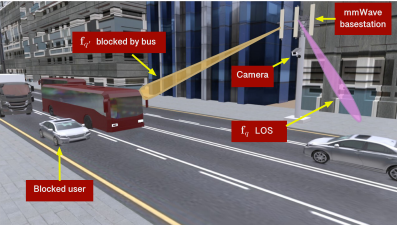
\includegraphics[width=0.7\linewidth]{figures/urban_scenario}
    \caption[mmWave base station equipped with camera to monitor LoS obstruction to users]{mmWave base station equipped with camera to monitor LoS obstruction to users \cite{Block_predict}.}
    \label{fig:urban_scenario}
\end{figure}

Within 6G, integrating mobile Base Stations (BSs) will be an enabler for achieving ubiquitous, network connectivity.
Radio Access Networks (RANs), consisting of mobile BSs, offer a dynamic and on-demand deployment approach, promising to meet varying Quality of Service (QoS) requirements in diverse contexts.
However, taking advantage of the full potential of mobile BSs requires developing software applications that can optimize RAN management.
In this context, leveraging xApps and rApps, defined by the O-RAN architecture, is a promising approach to optimize RANs and facilitate the integration of radio, sensing and vision-based information.

This approach paves the way for perception-aided mobile RANs, where real-time environmental awareness can overcome challenges in signal propagation and locating mobile devices that seek wireless connectivity.
In this context, Computer Vision (CV) is expected to enhance networks with capabilities beyond traditional telecommunications systems.
Using multiple sensors and video cameras, real-time environmental awareness may become a cornerstone for network optimization.
For that purpose, state-of-the-art CV algorithms may take charge of tasks related to processing and interpreting visual data while proactively identifying obstacles to prevent signal attenuation and blockage.
This convergence of CV and communications represents a promising advancement, holding the potential for improved heightened responsiveness, adaptability, and overall network performance.

\section{Motivation and Problem}\label{sec:motivation-and-problem}

In the ongoing evolution of mobile networks, successive generations have expanded connectivity capabilities while introducing heightened complexity.
This complexity, along with a growing dependence on closed, proprietary solutions, represents a significant challenge to integrating diverse technologies.
Recognizing these limitations is crucial, leading to the emergence of the 6G paradigm as a revolutionary response.
This paradigm envisions an evolution from closed systems to open-source implementations with open interfaces, where mobile networks complexity is managed through interoperable solutions.
The 6G paradigm stands as a catalyst for change in wireless communications.

However, the 6G paradigm faces a new layer of complexity due to dynamic and moving obstacles,  which can compromise communications in high-frequency bands.
This complexity arises the shorter wavelengths, making signals more prone to attenuation when encountering obstacles.
Millimeter-wave signals struggle to penetrate solid structures such as walls and buildings, potentially causing signal blockages and coverage gaps in densely populated urban areas.
The presence of vehicular traffic, pedestrians, and other mobile entities in the network's coverage area creates ephemeral shadowing effects, leading to signal blockages and fluctuations that directly impact wireless connectivity reliability.
This dynamism poses a considerable challenge to maintaining consistent signal strength and QoS levels, especially in areas with high vehicular or pedestrian density.
Addressing the dynamic nature of signal attenuation introduced by moving obstacles requires adaptive solutions, advanced signal tracking, predictive algorithms, and real-time adjustments in network configuration.

Furthermore, the distinction between LoS and Non-Line-of-Sight (NLoS) propagation paths adds to the challenge.
LOS paths, with a direct, unobstructed line between the transmitter and receiver, typically offer the most reliable and efficient communications.
However, in urban environments, NLoS paths, where signals reflect off buildings or scatter due to obstacles, become prevalent.
These NLoS paths introduce additional challenges, such as multipath fading and increased signal attenuation, further exacerbating connectivity issues.

A promising solution to the wireless communications challenges faced in densely populated urban areas lies in obstacle-aware networks, that leverage CV to extract information from video data.
By integrating CV algorithms, wireless networks can recognize and proactively overcome the challenges posed by moving obstacles.
This approach holds the potential to ensure uninterrupted communications and foster a seamless network experience in urban environments, aligning with the vision set forth by the 6G paradigm.

\section{Objectives}\label{sec:objectives}

The main objective of this dissertation was to implement vision-based RAN. This solution provides a Base Station to with environmental real-time perception provided by vision-based information.

In order to achieve this goal, specific objectives were defined:

    \begin{itemize}
    
    \item Implement a mechanism for detecting and tracking objects within the gNB's operational environment, enhancing the gNB's ability to adapt to dynamic environments.
    
    \item Develop a solution that extracts relevant information from video, through Computer Vision.
    This solution should provide information to the mobile network in real time to enhance the gNB's perception and obstacle awareness capabilities.
    
    \item Create a set of messages with information inferred from real-time video.
    This set should be relevant in the context of mobile networks, particularly for use by the gNB\@.
    These messages should be compliant with the O-RAN architecture.
    
    \item Develop an algorithm, implemented as an xApp, capable of receiving video-extracted information and RAN metrics to provide environmental perception for a RAN node.
      
    \item Validate and evaluate the proposed solution in reference networking scenarios.
    
    \end{itemize}

\section{Contributions}\label{sec:contributions}

The main contributions are the following:

    \begin{itemize}
    
    \item The introduction of video-based information into a 5G network, based on O-RAN architecture.
    This solution extracts relevant information from video feeds, tailored to indoor 5G use case.
    This is possible due to the development of a set of structured messages containing video-extracted information.
    These messages are specifically designed for improving network performance and obstacle management of the gNB\@.
    
    \item A xApp that processes video-extracted information and RAN metrics to determine optimal placement and configuration for a RAN\@.
    This application enhances the gNB's capabilities by enabling it to make informed decisions based on real-time environmental perception.
    
    \item The validation and evaluation of the performance of the proposed solution in a reference networking scenario.
    This includes a proof-of-concept for evaluating vision-aided networking solutions.
    
    \end{itemize}


% adjust references to chapters
\section{Document Structure}\label{sec:document-structure}

This document follows a structured approach.
Chapter~\ref{ch:state-of-the-art} discusses state-of-the-art and related work, addressing concepts related with to the challenges tackled in this dissertation.
Chapter~\ref{ch:specs_design_implem} outlines the proposed solution, detailing the system's specifications, design choices, and implementation.
Chapter~\ref{ch:validation} presents the experimental tests conducted to validate and evaluate the implementation of the proposed solution.
Finally, Chapter~\ref{ch:conclusion} synthesizes findings, draws conclusions, and provides directions for future work.
    \chapter{State of the art}\label{ch:state-of-the-art}

In this chapter, the fundamental concepts and existing solutions related to the problem of
this dissertation are presented.
Section \ref{sec:6g_charac} introduces 5G and 6G, addressing target performance requirements, emerging technologies, and envisioned applications.
It also briefly compares 5G and previous generations of mobile networks. In Section \ref{sec:5g_arch}, the main components and interfaces of the 5G architecture are presented and explained. In Section \ref{sec:RAN}, different RAN deployment approaches are explored and compared, including O-RAN. The O-RAN architecture and its specifications are presented with greater emphasis in Section \ref{sec:ORAN}. Section \ref{sec:CV} presents an overview of state-of-the-art tools used for the detection and tracking using Computer Vision. Section \ref{sec:rel_work} describes different solutions leveraging video sensing for wireless networks. Section \ref{sec:CONVERGE} discusses the objectives and architecture of the CONVERGE project. Finally, Section \ref{sec:Summary_SOA} summarizes the content of this chapter.

\section{5G and 6G Characterization} \label{sec:6g_charac}
The evolution from 4G to 5G represented a substantial advancement in mobile communications standards, addressing the limitations posed by the surge in connected devices and emerging technologies like the Internet of Things (IoT) and augmented reality (AR). The demand for faster and more reliable connectivity motivated the development of 5G, introducing higher frequency bands, wider channel bandwidths, and advanced antenna designs \cite{5G_apps}.

In the 6G paradigm, evolution is set to be even more transformative. 6G aims to surpass 5G in data rates, latency, and connectivity, as shown in Figure~\ref{fig:6g_capab}. The 6G design effort has already begun. The International Telecommunication Union (ITU) has advanced the development of 6G mobile technologies by publishing the framework for standards and radio interface technologies, known as Recommendation ITU-R M.2160-0,  \cite{ITU_2160-0} confirming the name for the next generation of IMT (“6G”) to be “IMT-2030”. This document introduces the expected capabilities of 6G technology and envisioned usage scenarios. This includes immersive communications, hyper-reliable and low-latency communications for industrial applications, enhanced ubiquitous connectivity, massive communications for IoT, and integration with artificial intelligence \cite{6G_ITU}. The use of terahertz frequency bands and the integration of artificial intelligence for network optimization and management are also envisioned \cite{6G_ITU}. Quantum communications, a concept not fully realized in previous generations, may become a reality in 6G, providing unprecedented security for wireless communications \cite{6G_ITU}.

\begin{figure}[H]
    \centering
    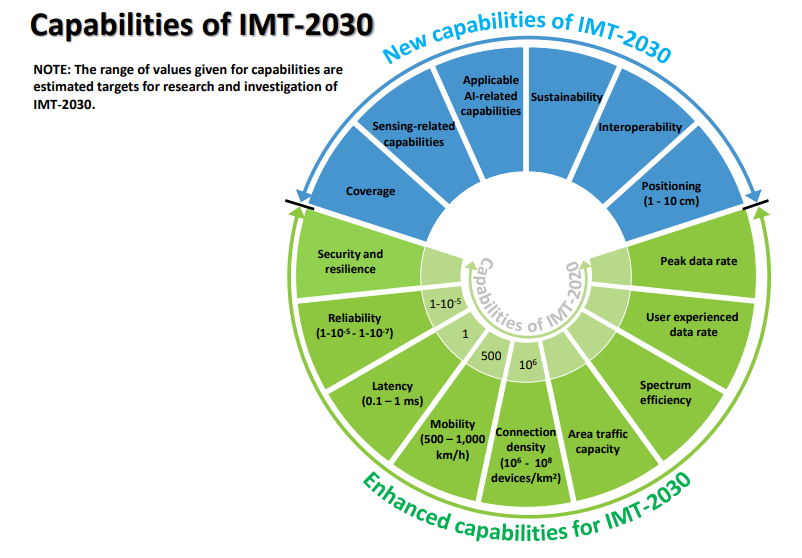
\includegraphics[width=0.8\linewidth]{figures/capabilities 6g.png}
    \caption[Capabilities of IMT-2030]{Capabilities of IMT-2030 \cite{ITU_2160-0}.}
    \label{fig:6g_capab}
\end{figure}

The proposed 6G applications include Unmanned Aerial Vehicle (UAV) networks, fully automated Vehicle-to-Everything (V2X), and holographic conferencing~\cite{6G_ITU}. These applications were initially envisioned for 5G but were only partially realized, emphasizing their priority in 6G development \cite{6G_ITU}. The predicted usage scenarios are depicted in Figure \ref{fig:6g_usage}.

5G networks have three main service categories that define the requirements and use cases for different types of applications. 6G is expected to extend those, depicted in Figure \ref{fig:6g_usage}: Enhanced Mobile Broadband (eMBB), Massive Machine Type Communications (mMTC), and Ultra-Reliable and Low Latency Communications (URLLC). 
\begin{itemize}
    \item \textbf{eMBB}: aims to provide a better user experience for mobile broadband services, such as video streaming, virtual and augmented reality, and online gaming. eMBB requires high data rates, high spectral efficiency, and wide coverage.
    \item \textbf{URLLC}: supports use cases that require strict quality of service levels, such as autonomous driving, remote surgery, and industrial automation. URLLC requires high reliability, low latency, and high availability.
    \item \textbf{mMTC}: enables various applications that collect and exchange data from sensors, meters, and machines, such as smart agriculture, smart city, and smart grid applications. mMTC requires high device density, low power consumption, and low data rates.
\end{itemize}

These three service categories are not mutually exclusive; some applications may require a combination. For example, a smart factory may need eMBB for high-definition video surveillance, mMTC for monitoring and controlling machines, and URLLC for real-time feedback and coordination. 

\begin{figure}[H]
    \centering
    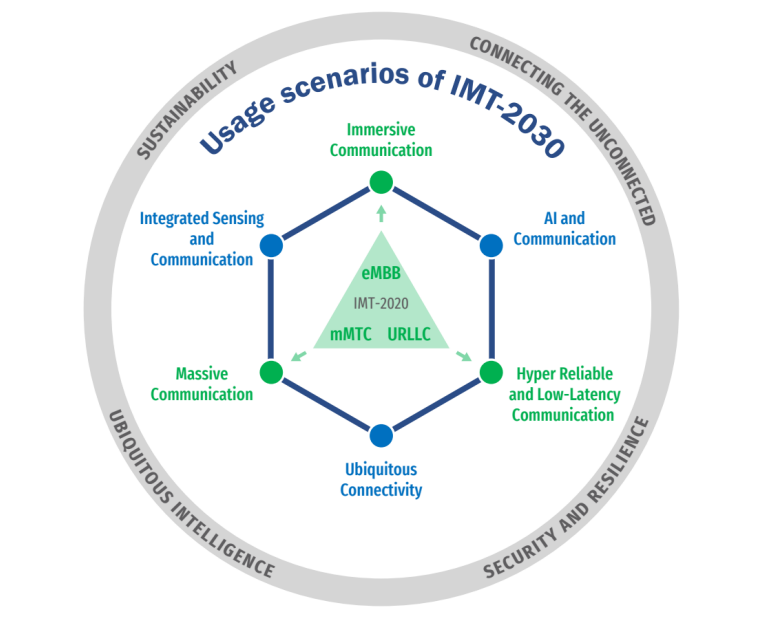
\includegraphics[width=0.5\linewidth]{figures/usage 6g.png}
    \caption[Usage scenarios and overarching aspects of IMT-2030]{Usage scenarios and overarching aspects of IMT-2030 \cite{ITU_2160-0}.}
    \label{fig:6g_usage}
\end{figure}

In 6G, progress is not only focused on enhancing data rates and connectivity. The shift towards open-source frameworks is a pivotal aspect, driven by the recognition that collaborative, community-driven development accelerates the evolution of network technologies \cite{6G_SOA}. This open-source paradigm aims to create a more inclusive, adaptable ecosystem where diverse contributors shape the future of wireless communications \cite{6G_SOA}.


\section{5G Architecture} \label{sec:5g_arch}

Considering the ongoing evolution and yet-to-be-fully-defined nature of the 6G architecture, this dissertation will utilize the established framework of 5G. The 3rd Generation Partnership Project (3GPP) stands behind the evolution of mobile communication standards \cite{3GPP_about_us}. The 5G New Radio (NR) architecture, a 3GPP standardization, embodies this commitment. By embracing the principles of Software Defined Networking (SDN), 3GPP enhanced wireless communications into scalability and flexibility. The strategic division of the control and data planes facilitates dynamic adaptability, empowering networks to respond to evolving demands and optimize resource utilization quickly.

The 3GPP model design maximizes interoperability with legacy infrastructure and equipment, promising an end-to-end ecosystem capable of supporting various use cases. A high-level architecture of 5G NR is presented in Figure \ref{fig:5G_arch}.

\begin{figure}[H]
    \centering
    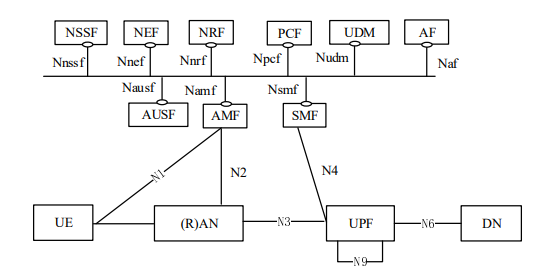
\includegraphics[width=0.7\linewidth]{figures/5g NR.png}
    \caption[High-level 5G NR Architecture]{High-level 5G NR Architecture \cite{ETSI_5G_NR}.}
    \label{fig:5G_arch}
\end{figure}

There are several relevant components in 5G NR, each playing a role in offering high-speed, low-latency connectivity for diverse applications and services. The User Equipment (UE) is at the forefront, including smartphones, IoT devices, and user terminals connected to the 5G network. The Radio Access Network (RAN) employs techniques, including Massive MIMO and beamforming, to optimize the performance of wireless communications established between UEs and the Core network. It employs a base station, also called gNodeB (gNB).

Within the Core network, the Access and Mobility Management Function (AMF) oversees access and mobility, ensuring a seamless and dynamic user experience. The Authentication Server Function (AUSF) guarantees secure user authentication, adding a layer of robustness to the network's security infrastructure. The Network Slice Selection Function (NSSF) assists in selecting appropriate network slices based on service requirements, tailoring the network to specific needs.

Other components include the Network Exposure Function (NEF), the enabler for exposing network assets and services to external applications. The Network Repository Function (NRF) maintains a repository of critical network information, contributing to the network's overall intelligence. The Policy Control Function (PCF) manages policy enforcement and control, including Quality of Service (QoS) and network slicing policies that define the user experience. The Unified Data Management (UDM) handles subscriber data. The Application Function (AF) oversees application-specific functions, enriching the user experience with tailored capabilities. Finally, the User Plane Function (UPF) manages user data traffic, and the Data Network (DN) allows the connection of the UPF to external data networks. These entities ensure efficient resource utilization and enhance the network's capabilities.

\section{RAN Deployment Approaches} \label{sec:RAN}
The traditional deployment of RANs involves strategically placing base stations and network infrastructure to enable wireless communications between UEs and the Core network, using radio signals for wireless connectivity.

In the conventional RAN deployment model, the Base Band Unit (BBU) and Remote Radio Unit (RRU) are central entities. The BBU manages the base station and ensures connectivity with the Core network, while the Remote Radio Head (RRH), connected to the base station's antenna, enables radio communication. Figure  \ref{fig:rru_bbu} depicts this deployment approach. 

\begin{figure}[H]
    \centering
    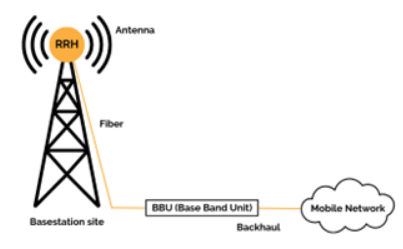
\includegraphics[width=0.5\linewidth]{figures/RRU_BBU.png}
    \caption[Traditional RAN deployment approach]{Traditional RAN deployment approach \cite{Trad_RAN}.}
    \label{fig:rru_bbu}
\end{figure}

Despite its widespread adoption, this approach faces several challenges, including concerns about achieving uniform coverage across diverse terrains, meeting the escalating demand for high data rates, and accommodating the increasing number of connected devices.

Network equipment providers typically design RAN implementations based on closed systems, lacking compatibility with equipment from other providers. This limitation forces network operators to rely on solutions from a single equipment provider, abdicating flexibility and interoperability. However, deploying and maintaining a network of physical base stations is a significant expense. In addition, the potential for interference between adjacent cells poses challenges to spectrum efficiency and overall network performance, particularly as the number of deployed base stations increases. Finally, adapting or expanding the network to meet growing user demands or technological advancements becomes a complex and time-consuming task within the traditional RAN deployment model.

Several solutions have emerged to address the challenges posed by traditional RAN deployments, offering enhanced flexibility, scalability, and efficiency. These solutions are based on softwarization and virtualization, utilizing the principles of Network Function Virtualization (NFV) and SDN. An alternative solution is the implementation of Cloud RAN (cRAN). By centralizing the BBUs in cloud data centers, this architecture introduces a more dynamic and adaptable approach to RAN deployment, as shown in Figure \ref{fig:cRAN}. The data centers, interconnected with RRUs in base stations through fronthaul interfaces, host virtualized BBUs aggregated in a pool and executed on a single machine. cRAN leverages Cloud computing principles to enhance scalability and resource optimization. This setup offers advantages such as capacity load balancing and heightened signal processing capabilities. However, C-RAN still faces the challenge of vendor lock-in, as systems and interfaces rely on proprietary implementations, which limits interoperability.

\begin{figure}[H]
    \centering
    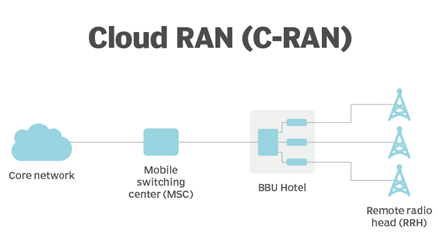
\includegraphics[width=0.5\linewidth]{figures/cRAN.png}
    \caption[cRAN deployment approach]{cRAN deployment approach \cite{cRAN}.}
    \label{fig:cRAN}
\end{figure}

Virtual RAN (VRAN) introduces a distinct approach for RAN deployment, leveraging NFV principles. In contrast to cRAN, which centralizes baseband processing on proprietary hardware, VRAN considers a virtualized model. This involves the replacement of specialized hardware with Commercial Off-the-shelf (COTS) hardware, providing a platform for deploying BBU nodes. However, the interfaces between the RRU and the virtualized BBU remain closed, and the interoperability challenge is not fully addressed.


To address the interoperability challenge, the 3GPP has created a disaggregation of the gNB into a gNB Central Unit (gNB-CU) connected to one or more gNB Distributed Units (gNB-DUs) via the F1 interface, as depicted in Figure \ref{fig:gnbdiss}. This disaggregation offers a standardized alternative, providing a more interoperable solution. The gNB-CU and gNB-DUs, while distributed, ensure effective communications through standardized interfaces, overcoming the closed interface limitations of traditional VRAN deployments. This leads to compatibility between virtualized network functions from different vendors, promoting a more flexible and vendor-neutral RAN architecture.

\begin{figure}[H]
    \centering
    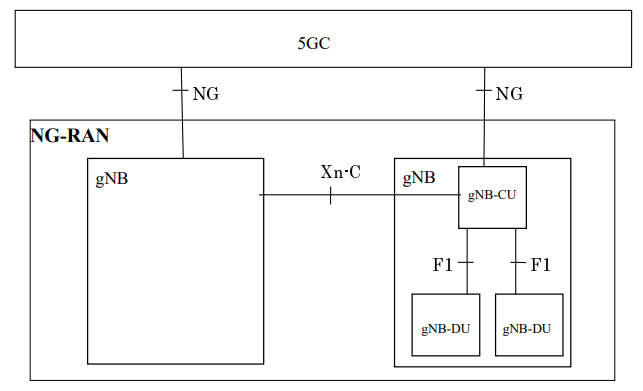
\includegraphics[width=0.6\linewidth]{figures/gnb_diss.png}
    \caption[Disaggregated gNB]{Disaggregated gNB \cite{gnb_diss}.}
    \label{fig:gnbdiss}
\end{figure}

The latest solution to these challenges is Open RAN (O-RAN). O-RAN represents a paradigm shift from traditional, closed RAN architectures, introducing openness and interoperability. This approach uses the disaggregated gNB previously mentioned and virtualization through COTS. O-RAN's main principle is to provide standardized interfaces, fostering interoperability between equipment from diverse providers. It promotes innovation and addresses the interoperability issues prevalent in closed systems. By embracing O-RAN, network operators can choose components based on performance, cost, and targeted use cases. This approach significantly reduces vendor lock-in, allowing for a more dynamic and cost-effective RAN deployment. The following section focuses on O-RAN, central to this dissertation's solution. 


\section{O-RAN Architecture}\label{sec:ORAN}
At the core of O-RAN's initiatives is the development of its reference architecture, depicted in Figure \ref{fig:ORAN}, which defines open interfaces and specifications. This section discusses the O-RAN architecture; it is divided into   Subsection \ref{sec:Components} for the key components and Subsection \ref{sec:Interfaces} for the interfaces of O-RAN. 
 
\begin{figure}[H]
    \centering
    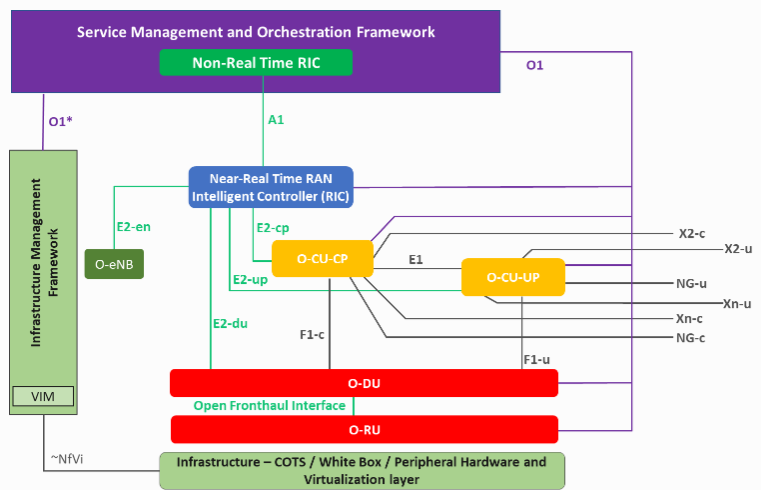
\includegraphics[width=0.6\linewidth]{figures/ORAN.png}
    \caption[O-RAN architecture overview]{O-RAN architecture overview \cite{ORAN-ARCH}.}
    \label{fig:ORAN}
\end{figure}

\subsection{O-RAN Components}\label{sec:Components}
The O-RAN architecture comprises several key components, each serving a specific function to enhance network performance and promote openness and interoperability. The Centralized Unit Control Plane (O-CU-CP) and the Centralized Unit User Plane (O-CU-UP) are integral parts of the O-RAN architecture. The O-CU-CP handles the centralized control plane functions, enabling efficient coordination and management of radio resources. On the other hand, the O-CU-UP focuses on user plane functions, dealing with the processing and forwarding user data. The O-CU-CP implements higher layers of the 3GPP protocol stack, such as the Radio Resource Control (RRC) layer, managing the connection life cycle. The O-CU-UP also implements the higher layers of the 3GPP protocol stack. However, it manages the Quality of Service (QoS) of the traffic flows and handles reordering packet duplication and encryption for the wireless interface. They can both be deployed in the Cloud or at the Edge of the network and can communicate with multiple O-DUs and O-RUs.

The Distributed Unit (O-DU) decentralizes the baseband processing functions. It collaborates with the Radio Unit (O-RU), responsible for radio frequency transmission and reception. This separation of functions enhances scalability, allowing for more flexible and efficient resource allocation. The O-DU implements the lower layers of the 3GPP protocol stack, such as the Radio Link Control (RLC) layer, the Medium Access Control (MAC) layer, and part of the physical layer. It can be virtualized on servers at the Edge of the network, connecting to one or more O-RUs through the O-RAN Open Fronthaul interface. The O-DU also interacts with the near-Real-Time Radio Intelligent Controller (Near-RT RIC) through the E2 interface, enabling data-driven closed-loop control and optimization of the RAN.

The O-RU implements the remaining part of the physical layer and the Radio Frequency (RF) components. It is usually deployed close to the antennas, connecting to one or more O-DUs through the O-RAN Open Fronthaul interface. The O-RU performs time-domain functionalities, such as precoding, Fast Fourier Transform (FFT), cyclic prefix addition/removal, and beamforming.

Near-RT RIC and Non-Real-Time (Non-RT) RIC introduce intelligence and automation into the O-RAN ecosystem. The Near-RT RIC manages and controls the RAN at Near-real-time (10 ms to 1 s) time scale. It is deployed at the Edge of the network, interacting with multiple O-DUs and O-CUs through the E2 interface. The Near-RT RIC hosts multiple applications, called xApps, which implement custom logic for RAN optimization and control. In contrast, the Non-RT RIC manages and controls the RAN at non-real-time (more than 1 s) time scale. It is part of the Service Management and Orchestration (SMO) framework, complementing the Near-RT RIC for intelligent RAN operation and optimization. The Non-RT RIC hosts multiple applications, called rApps, providing value-added services to support and facilitate RAN optimization and operations.

\subsection{O-RAN Interfaces} \label{sec:Interfaces}

The O-RAN architecture relies on multiple interfaces that enable seamless communications, control, and data exchange among diverse components of O-RAN. These open interfaces ensure interoperability, flexibility, and efficient orchestration within the RAN ecosystem.

One crucial interface is the E2 interface, which establishes a connection between the Near-RT RIC and the RAN nodes, including the Centralized Unit (CU) and Distributed Unit (DU). Through the E2 interface, the Near-RT RIC gains access to data from the RAN, enabling informed decision-making and facilitating the transmission of control actions and policies to optimize RAN performance. The E2 interface supports various message types, such as subscription, indication, control, and policy, contributing to the dynamic adaptability of the RAN.

The A1 interface enables communications between the non-RT RIC and the Near-RT RIC. It is responsible for policy guidance and enrichment. This interface allows the non-RT RIC to provide valuable insights and receive feedback and status reports from the Near-RT RIC. By supporting message types like policy type, policy instance, and service model, the A1 interface fosters cooperation between different RIC components, enhancing overall RAN intelligence.

The O1 interface connects the SMO framework and the RAN nodes (CU, DU, and RU). It empowers the SMO to perform essential functions, including configuration, fault management, performance monitoring, and security management of the RAN elements. With support for various message types, such as configuration, fault, performance, and security management messages, the O1 interface ensures efficient and centralized management of the RAN.

The O-RAN Open Fronthaul interface establishes a critical link between the DU and the RU, facilitating the exchange of user and control plane data. Additionally, it enables the DU to configure and manage the RU functionalities. Built on top of the eCPRI and IEEE 1914.3 standards, this interface supports different message types, including user plane, control plane, synchronization plane, and management plane messages, ensuring a flow of information between the DU and RU.

Finally, the O2 interface serves as a bridge between the SMO and the O-Cloud. This interface empowers the SMO to orchestrate and manage virtualized network functions hosted on the O-Cloud platform. With support for diverse message types, including inventory, monitoring, provisioning, fault tolerance, and update messages, the O2 interface facilitates the efficient coordination and deployment of virtualized network functions.

The O-RAN architecture promotes cooperation and innovation across the ecosystem, allowing network operators to seamlessly integrate components from different vendors. This open and interoperable approach fosters competition, accelerates technological evolution, and empowers operators to tailor their networks according to specific requirements. The O-RAN Alliance's role in standardization efforts is essential in guaranteeing consistency and compatibility across the diverse elements of the O-RAN architecture.


\subsubsection{E2 Interface}\label{sec:protocols}
As mentioned previously, the E2 interface connects the Near-RT RIC to the E2 nodes.
The interaction between those entities is defined by the E2 Service Model (E2SM).
Each E2SM model defines a service that a RAN function can perform.
The basic actions are: report, insert, control and policy.
Each of these is transported through E2 Application Protocol (E2AP) procedures.

For instance, a report contains information from the E2 nodes to the RIC/xApps.
An xApp sends an E2AP subscription for requesting a report.
The E2SM specifies the types of reports that can be sent and trigger the events necessary.
Then, the RAN function sends an E2SM report transported through a E2AP Indication Message.

Thus, the E2 interface uses the E2 Application Protocol (E2AP) to handle signaling and control procedures.
E2 Service Models (E2SMs) define the specific application-level data and control exchanges, together enabling the Near-Real-Time RAN Intelligent Controller (Near-RT RIC) to efficiently interact with and manage RAN functions in a standardized and customizable manner.

The protocol stack of this interface is depicted in Figure~\ref{fig:E2_stack}.

\begin{figure}[H]
    \centering
    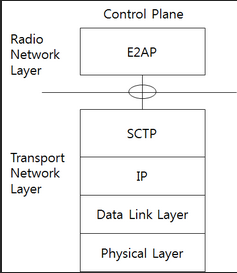
\includegraphics[width=0.3\linewidth]{figures/E2_stack}
    \caption[E2 protocol stack]{E2 protocol stack \cite{E2GAP}.}
    \label{fig:E2_stack}
\end{figure}

The E2AP messages are encoded in Abstract Syntax Notation One (ASN.1) Basic Packed Encoding Rules (BASIC-PER) Aligned Variant.
The encoding rules are defined in ITU-T Rec. C.691~\cite{ITU_T_C691}.
ASN.1 is a standard interface description language for defining data structures that can be serialized and deserialized in a cross-platform way.

The E2AP services are categorized into two groups: RIC Functional Procedures and Global Procedures.
The RIC Functional Procedures include actions used to pass application-specific messages between Near-RT RIC applications and a target RAN function in an E2 node.
The RIC Functional Procedures are designed to handle application-specific messaging.
These procedures facilitate the communication between Near-RT RIC applications and a target RAN function within an E2 node.
They include:

\begin{itemize}
\item RIC Subscription: Enabling the Near-RT RIC to subscribe to specific events or data from the RAN functions.
\item RIC Indication: Allowing the RAN functions to send reports or indications to the Near-RT RIC based on the subscribed events.
\item RIC Control: Permitting the Near-RT RIC to send control messages to manage and influence the behavior of the RAN functions.
\end{itemize}
These functional procedures ensure adaptive and real-time management of the RAN, providing mechanisms for monitoring, reporting, and controlling various aspects of the network.

In contrast, the Global Procedures are utilized for operations that do not directly relate to a specific application but are essential for the overall management and maintenance of the E2 interface.
They include:

\begin{itemize}
\item E2 Setup: Establishing the initial configuration and setup of the E2 interface between the Near-RT RIC and the E2 nodes.
\item E2 Configuration Update: Updating the configuration parameters of the E2 interface as required by changes in the network or operational policies.
\item E2 Reset: Handling the reset operations to recover from error conditions or to reinitialize the E2 interface.
\end{itemize}
These global procedures ensure that the E2 interface is capable of handling various network scenarios and requirements.



\section{Computer Vision-based detection and tracking solutions}\label{sec:CV}

CV, a branch of artificial intelligence, enables machines to interpret and make decisions based on visual data, involving the understanding and analyzing of images and videos. Object detection and tracking are tasks of CV, allowing machines to identify, locate, and monitor specific objects within visual content while facilitating recognition and comprehension of real-world scenarios.CV is used in various domains. In autonomous vehicles, object detection and tracking tasks ensure safe navigation by identifying pedestrians, vehicles, and obstacles. Retail uses CV for automated checkout and inventory management, while security systems employ it for real-time monitoring and tracking of suspicious activities. Augmented reality relies on CV to seamlessly integrate virtual elements into the real world.

In mobile networks, object detection and tracking may play a key role in optimizing network performance. They may allow for analyzing user behavior patterns, helping telecom providers to enhance coverage and capacity in areas with high user density. In the context of 5G networks, obstacle-aware networks utilize object detection and tracking to improve communications efficiency and reliability in the presence of obstacles. Object detection and tracking allow identifying and categorizing obstacles while enabling dynamic adjustments of network parameters for optimized signal strength and connectivity. Integrating vision-based capabilities in 5G systems paves the way to enable proactive responses to environmental changes, mitigating signal blockage and enhancing overall communications quality. Overall, object detection and tracking contribute to improved network performance, efficient maintenance processes, and an enhanced user experience in the mobile telecom sector.

This section is further divided into three sections. Section \ref{sec:detect} discusses the state-of-the-art detection models. Section \ref{sec:track} discusses the tracking solutions. Finally, Section \ref{sec:open_tools} evaluates the existing open-source tools, their applicability, and their relevance to the specific challenges addressed in this dissertation.

\subsection{Detection models}\label{sec:detect}

Object detection models are essential in locating and classifying objects within images, utilizing bounding boxes and labels. Generic object detectors, foundational in CV, exist in two main types: two-stage and one-stage detectors. Two-stage detectors, exemplified by Faster Region-based Convolutional Neural Network (Faster R-CNN) \cite{FasterRCNN}, lie in a traditional approach of proposing regions of interest (RoIs) before classifying and refining them. This method prioritizes accuracy but may have longer processing times. On the other hand, one-stage detectors, such as You Only Look Once (YOLO) \cite{YOLO} and Single Shot MultiBox Detector (SSD) \cite{SSD}, optimize the process by predicting bounding boxes and class probabilities in a single pass, prioritizing real-time performance. These detectors are versatile and crucial in applications like image recognition and can be applied to diverse scenarios. Figure \ref{fig:1vs2} depicts the differences in the architecture of one-stage and two-stage detectors.

\begin{figure}[H]
    \centering
    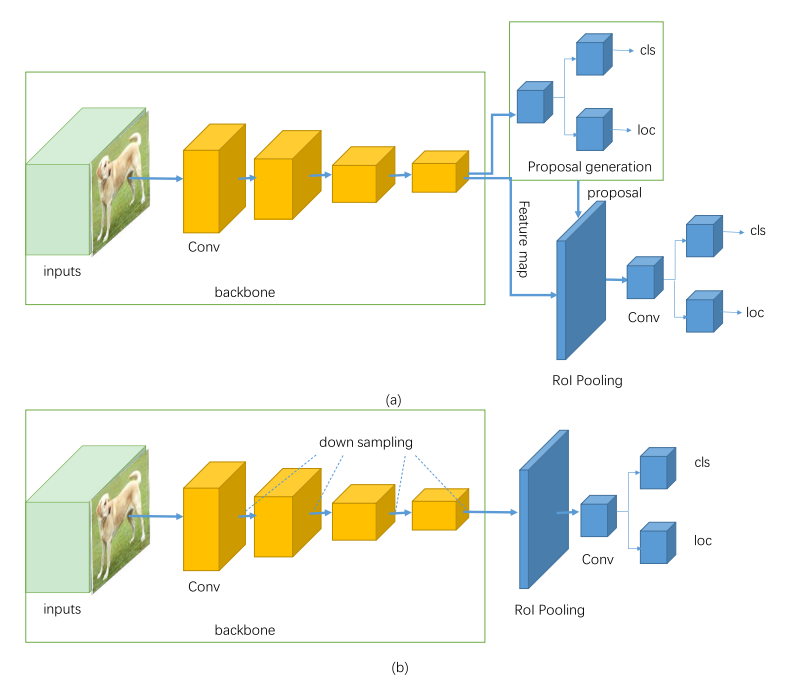
\includegraphics[width=0.6\linewidth]{figures/single vs two.png}
    \caption[Two stages vs. single stage detector architecture]{Two stages vs. single stage detector architecture. (a) Exhibits the basic architecture of two-stage detectors, and (b) shows the basic architecture of one-stage detectors \cite{1vs2}.}
    \label{fig:1vs2}
\end{figure}

In the case of two-stage detectors, as depicted in Figure \ref{fig:1vs2} (a), the architecture involves a region proposal network (RPN) in the initial phase. The RPN takes input images and generates region proposals or bounding boxes that are likely to contain objects of interest. These proposals are then fed into a classifier and regressor for further processing. The classifier determines the object's class within each proposed region, while the regressor refines the coordinates of the bounding boxes. This two-stage approach allows for systematic and staged input processing, providing a more detailed analysis that often leads to improved accuracy.

Conversely, Figure \ref{fig:1vs2} (b) illustrates the basic architecture of one-stage detectors. In this case, the detector predicts bounding boxes directly from the input images without needing a separate region proposal network. The architecture involves a series of convolutional layers forming a backbone network. The yellow cubes represent these convolutional layers, organized into blocks with the same resolution. Due to down-sampling operations after each block, the subsequent cubes gradually decrease in size. The thick blue cubes, consisting of convolutional layers, handle the final prediction, including object classification and bounding box regression. Notably, the flat blue cube represents the RoI pooling layer, which generates feature maps for objects of the same size. This one-stage approach prioritizes simplicity and speed, making it particularly efficient for real-time applications, though it may face challenges in accurately detecting small or occluded objects.


The decision between single-shot and two-shot detectors involves balancing speed, accuracy, and complexity. Single-shot detectors like YOLOv3 \cite{YOLOv3} process images in a single pass, prioritizing speed and simplicity without a separate Region Proposal Network (RPN). This means that single-shot detectors employ one module comprising both tasks instead of having separate modules in the architecture for the RPN and the Classification and Regression Heads. For this reason, they are simple to train and deploy but may sacrifice accuracy, especially for small or occluded objects. In contrast, two-shot detectors like Faster R-CNN improve accuracy and reliability by employing a region proposal network and a separate classification network. They handle complex scenes and small objects efficiently but are slower, more complex, and computationally intensive. The choice between the two detectors hinges on the application's specific needs, requiring the consideration of trade-offs between speed and accuracy.


\subsection{Tracking models}\label{sec:track}

Regarding deep learning-based object tracking, the methods can be classified into three distinct categories, each leveraging deep neural networks for enhanced tracking performance. Firstly, deep network features-based methods enhance tracking by utilizing semantic features extracted from deep Convolutional Neural Networks (CNNs). These methods employ various approaches to learn affinities between detections and track-lets, incorporating techniques such as multiple hypothesis tracking, Siamese networks, or optical flow features. An example of this is the Siam R-CNN \cite{siam}. It has applications in scenarios where precise and robust object tracking is required, including in surveillance systems for accurate monitoring of individuals or objects. However, the computational complexity of Siamese-based methods may make them less suitable for real-time applications on resource-constrained devices within mobile networks. Another example in this category is Simple Online and Real-time Tracking with a Deep Association Metric (Deep SORT)\cite{DeepSORT}. Deep SORT extends the capabilities of the SORT algorithm \cite{SORT} by integrating deep learning techniques, specifically using deep features for association and tracking. This extension enhances the algorithm's ability to handle challenging scenarios such as occlusions and varying object appearances, making it valuable in real-time scenarios, including traffic monitoring or event surveillance within mobile networks.

Secondly, deep network embedding-based methods integrate deep CNNs as the central component of the tracking framework. These methods adopt different learning tasks, including discriminative, metric, or generative learning, to estimate parameters or distances for matching detections and track-lets. The discriminative Correlation Filter (DCF) trackers, such as the Kernelized Correlation Filter (KCF) \cite{KCF}, represent an influential category. These trackers leverage deep CNNs as integral components, employing discriminative learning tasks to estimate parameters for matching detections and track-lets. Their application extends to scenarios where a balance between accuracy and real-time performance is essential, including in video analysis for content creation, in which tracking objects efficiently contributes to the overall editing process.

Finally, end-to-end deep network learning-based methods take a direct approach by using deep networks to output tracking results without relying on intermediate steps. These methods leverage diverse architectures, such as Recurrent Neural Networks (RNNs), Long Short-Term Memory Networks (LSTMs), and attention mechanisms, to model the temporal dependencies and dynamics of the tracked objects. Algorithms like LSTM trackers and Attention-based trackers demonstrate the effectiveness of direct end-to-end approaches. LSTMs demonstrate effectiveness in applications requiring temporal understanding, benefiting video-based tasks such as action recognition or gesture tracking. However, the resource-intensive nature of LSTMs may impact real-time performance, making them less suitable for deployment in mobile networks with limited computational resources. On the other hand, Attention-based trackers, exemplified by algorithms like ATOM, offer efficient solutions for applications demanding real-time visual attention, such as augmented reality experiences on mobile devices. 

While concepts of CV are discussed in this subsection, it is important to note that the specific exploration of dedicated object detection algorithms tailored for distinct applications will not be covered in this context. The focus remains on the fundamental principles, applications, and the broader scope of object detection and tracking within the generic object detectors. Specialized algorithms designed for specific applications, while integral to the field, ensure in-depth discussions tailored to their unique contexts and use cases, which may extend beyond the scope of this work. More extensive research on state-of-the-art object detection and tracking can be found at \cite{obj_detec_SOA}.

\subsection{Open-source Tools}\label{sec:open_tools}
In object detection and tracking, open-source tools are essential in providing accessible and adaptable solutions. Integrating these tools into a gNB based on the O-RAN architecture in real-time applications requires careful consideration of speed, accuracy, and compatibility. Two notable tools mentioned previously stand out for their effectiveness: YOLO and BoT-SORT.

YOLO has gained attention in both academic research and practical applications. YOLO's one-shot detection approach is foundational to its success, as it processes the entire image in a single pass. This approach is particularly advantageous for applications demanding low latency, making it a compelling choice for integration within an O-RAN architecture. Table \ref{tab:yolo_performance} presents a comparison made in \cite{YOLO_compare} based on mean Average Precision (mAP) and frames-per-second (fps) between different YOLO models to run a video on CPU and GPU, proving the evolution of the algorithm. 

The mAP summarizes the classification performance of the object detection model across different categories, while the fps assesses the real-time performance of a model.

\begin{table}[H]
    \caption[Performance Metrics of Various YOLO Versions]{Performance Metrics of Various YOLO Versions \cite{YOLO_compare}.}
    \label{tab:yolo_performance}
    \centering
    \begin{tabular}{|l|l|l|l|l|l|}
        \hline
        Versions & mAP & CPU fps & GPU fps & CPU time (s) & GPU time (s) \\ \hline
        YOLOv3 & 33.2 & 2.88 & 37 & 324.539 & 14.625 \\
        YOLOv4 & 57.8 & 1.21 & 28.9 & 568.484 & 16.458 \\
        YOLOv4-tiny & 38.1 & 18.46 & 65.8 & 46.751 & 13.351 \\
        YOLOv5-nano & 28.0 & 6 & 40 & 87.168 & 15.536 \\
        YOLOvS-small & 37.4 & 4 & 36 & 152.821 & 18.187 \\
        YOLOv6-nano & 35.9 & 5.4 & 110.7 & 103.253 & 16.551 \\
        YOLOv6-small & 43.5 & 2.7 & 72.8 & 289.838 & 18.911 \\
        YOLOv6-tiny & 40.3 & 4.2 & 80.9 & 196.117 & 18.078 \\
        YOLOv7 & 66.7 & 0.76 & 42 & 970.85 & 16.075 \\
        YOLOv7-tiny & 53.4 & 3 & 50 & 201.78 & 12.955 \\ \hline
    \end{tabular}
\end{table}


Academic research has consistently recognized YOLO for its contributions to the CV field. The original YOLO paper \cite{YOLO} introduced a new approach to object detection, achieving remarkable accuracy and speed. Since then, the YOLO architecture has undergone several iterations, each bringing improvements in terms of performance and usability.

\begin{figure}[H]
    \centering
    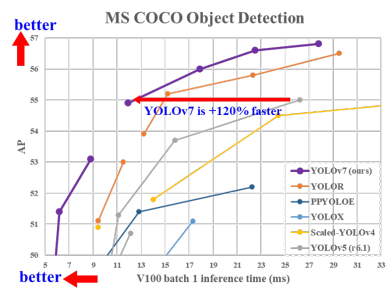
\includegraphics[width=0.6\linewidth]{figures/yolov7.png}
    \caption[Comparison between real-time object detectors]{Comparison between real-time object detectors \cite{yolov7}.}
    \label{fig:yolov7}
\end{figure}

One notable aspect of YOLO is its usability. The architecture is designed to be accessible, making it easier for researchers and developers to implement and experiment with object detection. The availability of pre-trained models further enhances the user experience, allowing practitioners to leverage the power of YOLO without an extensive background in deep learning.

The recent evolution of YOLO, including contributions from the Ultralytics \cite{ultralytics_docs} team, has further improved its performance. Ultralytics, a prominent contributor to YOLO's development, focuses on optimizing and advancing the capabilities of YOLO for real-world applications. Their efforts have resulted in performance improvements, enhanced training capabilities, and a user-friendly interface, making YOLO even more attractive for applications demanding real-time object detection, such as those encountered in O-RAN architectures. Figure \ref{fig:yolov7} compares real-time object detectors. Notice that, in the MS COCO dataset \cite{COCO}, the algorithm that performs best is YOLOv7. 

While all categories presented previously on section \ref{sec:track} of object tracking methods can potentially be employed for Multiple Object Tracking, deep network features-based approach will be presented further. SORT, a representative method in this category, is designed for efficient tracking by primarily relying on basic motion and position information to link detections across frames. Although effective under ideal conditions, SORT may struggle with challenges like appearance variations and occlusions due to its simplicity.

In response to these limitations, Bag of tricks for SORT based methods (BoT-SORT) has been developed. BoT-SORT uses semantic features extracted from deep CNNs, which increases proficiency in distinguishing between different classes of obstacles, such as vehicles and pedestrians, even in occlusions scenarios and varying appearances. This capability enables BoT-SORT to balance speed and accuracy, which makes it suitable for real-time tracking applications. 


\begin{figure}[H]
    \centering
    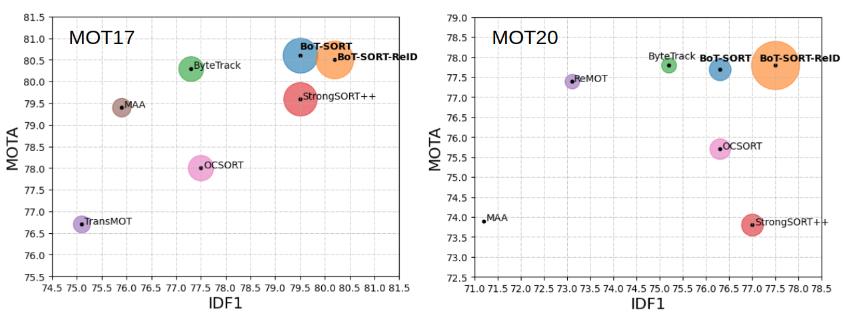
\includegraphics[width=0.6\linewidth]{figures/botsort.png}
    \caption[Comparison of state-of-the-art trackers in the MOT17 and MOT20]{ Comparison of state-of-the-art trackers in the MOT17 and MOT20\cite{botsort}.}
    \label{fig:botsort}
\end{figure}

Figure \ref{fig:botsort} compares trackers participating in the MOT17 and MOT20 challenges, highlighting the significant performance of BoT-SORT. The positioning of each tracker on the plot reflects its performance in terms of identification F1 Score(IDF1) on the horizontal axis and Multiple Object Tracking Accuracy (MOTA) on the vertical axis. Finally, the circle's radius around each point indicates its Higher Order Tracking Accuracy (HOTA) score.

The IDF1 measures the accuracy of identity assignments in tracking results, encompassing precision and recall of identity associations. A higher IDF1 score indicates a better ability to correctly associate detections with existing tracks while maintaining object identities over time. As for MOTA, it offers an overall assessment of tracking accuracy, considering various error sources such as false positives, false negatives, and identity switches. A higher MOTA score indicates superior tracking accuracy, as it penalizes tracking errors like missing detections and incorrect associations.  Finally, HOTA extends the evaluation beyond MOTA by incorporating additional information about the quality of track fragments. It considers the completeness, correctness, and assignment ambiguity of track fragments, providing a more nuanced evaluation of tracking performance.

The scores achieved by BoT-SORT demonstrate its effectiveness in accurately associating detections with tracks, maintaining object identities, and producing high-quality track fragments, making it a compelling choice for multiple object tracking tasks.

As presented in \cite{botsort}, BoT-SORT presents a 6.6 Frames Per Second (FPS) score. Considering the indoor scenario, this processing speed offers acceptable results for the intended application. In indoor environments, where the movement of objects is typically constrained and relatively slow compared to outdoor scenarios, BoT-SORT should perform well. This metric ensures that it can maintain real-time tracking capabilities in dynamic indoor environments.

The combination of acceptable performance metrics and a satisfactory FPS demonstrates the viability of BoT-SORT for indoor multiple object tracking applications. It indicates that BoT-SORT can reliably track objects in real-time indoor scenarios accurately.

Regarding implementation, BoT-SORT is one of the supported trackers within the Ultralytics YOLO framework. This choice offers benefits for object-tracking applications. BoT-SORT's integration with YOLO ensures improved tracking accuracy, efficient real-time processing, and seamless object ID management, facilitating detailed analytics and monitoring in video streams. Using BoT-SORT with Ultralytics' Python API enables quick deployment of tracking solutions. 

The selection of YOLO and BoT-SORT is justified by their strengths in speed, accuracy, and adaptability to real-time applications. Their integration into a video-based gNB within an O-RAN architecture aligns with the objective of efficient and reliable object detection and tracking in wireless communications networks.



\section{Related Work}\label{sec:rel_work}
In recent developments, a limited number of publications are exploring the integration of CV to enhance mobile networks, particularly within the framework of O-RAN.

In \cite{Block_predict}, a machine learning framework is proposed to enable proactivity in wireless networks, leveraging visual data captured by video cameras at base stations. The focus is on anticipating future blockages and facilitating user hand-offs in advance. The proposed two-component deep learning architecture, using YOLOv3 \cite{YOLOv3}, incorporates bimodal data, employing visual and radio information to predict blockages proactively and execute seamless user hand-offs. The results demonstrate the architecture's efficacy in accurately detecting blockages through experimentation, enhancing reliability, and reducing latency in the wireless network. The system model considers a small-cell millimeter-wave (mmWave) base station equipped with a uniform linear array and an RGB camera. The channel considers a geometric mmWave model with L clusters, and the authors provide a mathematical formulation for modeling signal blockage while defining Line-of-Sight (LOS) and Non-Line-of-Sight (NLOS) channels.
Moreover, they propose a future exploration based on the investigation of radar-based detection approaches to pinpoint the location of users who are served post-blockage. This approach holds the potential for predicting blockages in real network environments with multiple users. The proposed approach may be integrated with the O-RAN architecture, envisioning the implementation of the CU at the Near-RT RIC. This approach introduces potential enhancements to wireless networks' reliability and predictive capabilities.

A similar approach is presented in \cite{Block_predict2}. The authors employ CV to address challenges in mmWave wireless communications systems, specifically focusing on beam selection and blockage prediction. Employing a synergy between CV and deep learning tools, the study proposes an approach for predicting mmWave beams and blockages directly from RGB images captured by cameras and sub-6GHz channels. It eliminates the need for explicit channel knowledge or beam training. Two deep learning-based solutions are proposed, anchored in deep convolutional networks and transfer learning, with a foundational reliance on the 18-layer Residual Network (ResNet-18). This ResNet-18 model is tailored for beam prediction, treating the task as an image classification challenge while mapping images to beam indices from a codebook. Simultaneously, another ResNet-18 model, equipped with a customized fully connected layer, performs user detection as a binary classification task, contributing to determining link status based on user detection results and sub-6GHz channel information. The proposed approach shows the potential of CV and deep learning to revolutionize mmWave system capabilities, providing an innovative solution to address wireless communications challenges.

In \cite{CVAided}, a real-world evaluation of leveraging visual data and machine learning techniques is presented to predict mmWave dynamic link blockages proactively before they occur. Proactive prediction of LOS link blockages enables mmWave/sub-THz networks to implement preemptive network management actions, such as proactive beam switching and hand-off, prior to link failures. Such measures can significantly enhance network reliability and reduce latency while maximizing the efficient utilization of wireless resources. They assess the practical viability of this approach, developing a Computer Vision-based solution that processes visual data captured by a camera installed at the infrastructure node. Additionally, their proposed solution's viability is investigated using the DeepSense 6G \cite{deepsense} dataset, which encompasses multi-modal sensing and communication data. The results highlight the promising potential of integrating CV techniques in communications networks to mitigate link blockages and enhance network performance.

%--------

These works are part of a research group that developed DeepSense6G \cite{deepsense}, a real-world multimodal sensing and communication dataset. This dataset comprehends several scenarios utilizing various sensing approaches such as RGB cameras, radar, and LiDAR with applications in beam prediction, blockage prediction, positioning, and more. DeepSense6G is designed to facilitate research in multimodal sensing and wireless communication, offering data that supports developing and evaluating advanced algorithms.


In addition to DeepSense6G, there are other multimodal datasets that cater to different needs of the research community. For instance, the Vision-Wireless (ViWi) dataset \cite{ViWi} includes synchronized multimodal data from cameras, LiDAR, and wireless sensors, facilitating research in beamforming, user localization, and blockage prediction. The ViWi dataset utilizes advanced 3D modeling and ray-tracing software to generate high-fidelity synthetic data, ensuring that both visual and wireless data samples are accurately represented for the same scenes. By providing data that captures both visual and wireless signals, the ViWi dataset enables researchers to develop and validate algorithms that exploit the synergy between these modalities, leading to more robust and efficient communication systems. Notably, the ViWi dataset is parametric, systematic, and scalable, making it possible to generate training and testing datasets and a common ground for assessing the quality of different machine learning-powered solutions.

Another notable dataset is the Synthesia of Machines \cite{Synthesia}. This dataset leverages advanced simulation techniques to generate multimodal data, including visual, audio, and sensory information. The Synthesia of Machines dataset is particularly useful for training machine learning models in environments where collecting real-world data is challenging or impractical. By providing high-quality synthetic data, this dataset helps researchers overcome the limitations of real-world data collection, allowing for the development and testing of algorithms in a controlled and scalable manner. Synthetic data also facilitates exploring a wide range of scenarios and conditions, enhancing the robustness and generalizability of machine learning models. ViWi and Synthesia of Machines leverage simulation to provide data environments for algorithm development and testing. While the presented datasets enable significant advancements in multimodal sensing and have facilitated breakthroughs in various research areas, they still need to integrate with the ongoing efforts in the O-RAN architecture. 

%--------------

In the context of O-RAN deployments, \cite{xApps} introduces OpenRAN Gym, a framework tailored for data-driven experimentation within the OpenRAN ecosystem, focusing on intelligent closed-loop control. OpenRAN Gym enables the development, training, and testing of xApps, data-driven applications specifically designed for the near-RT RIC. The xApp design process integrates service models (SMs) for communications with RAN nodes over the E2 interface, incorporating data-driven logic units hosting AI/ML models for RAN inference and control. The framework's capabilities are exemplified through a compelling use case, considering an xApp that jointly manages scheduling and slicing functionalities of base stations based on real-time RAN data. Rigorous testing on the Colosseum wireless network emulator, featuring seven base stations and forty-two users, highlights xApp's adaptability to diverse traffic scenarios. The results emphasize the advantages of online fine-tuning, showcasing improved performance and generalization. OpenRAN Gym's contribution lies in its potential to revolutionize intelligent closed-loop RAN control through the innovative development and application of xApps. For these reasons, \cite{xApps} is an important reference for best practices integrating object detection algorithms with the O-RAN architecture.

% GOnçalo and David Maia thesis
Regarding mobile gNBs, the goals of this dissertation are aligned with those achieved by Gonçalo Queirós \cite{Goncalo} and David Maia \cite{David}. David Maia focuses on developing a private standalone on-demand 5G network, utilizing a 5G gNB carried by a mobile robotic platform. This setup provides connectivity for 5G mobile terminals. It incorporates an On-Demand Mobility Management Function (ODMMF) for monitoring radio conditions of served UEs and remotely controlling the mobile robotic platform in real-time using its video cameras.

Gonçalo Queirós, on the other hand, focuses on deploying a private Standalone 5G Network with a mobile RAN employing the O-RAN architecture. This approach leverages the standards and specifications proposed by the O-RAN Alliance to create open, interoperable networks based on independent virtualized components connected through standardized open interfaces. The mobile RAN consists of a 5G gNB carried by a Mobile Robotic Platform capable of autonomous positioning. The solution employs a novel Mobility Management xApp, which autonomously collects metrics from the RAN, analyzes them, and uses an algorithm to determine and control the placement of the mobile RAN to optimize connection quality between UEs and the gNB. This highlights the potential of the O-RAN architecture to facilitate the deployment of multi-vendor components and enhance the flexibility and efficiency of 5G networks.

The main differences between our work and theirs lie in introducing Computer Vision to the 5G network and working towards integrating content extracted from such tools into the O-RAN framework. While their work focused on developing the 5G Core network and leveraging NFV and SDN for scalability and manageability, our dissertation aims to enhance the O-RAN architecture by incorporating CV techniques. This integration allows for more intelligent and autonomous mobility management, enabling repositioning the mobile robotic platform based on visual data without user input. By merging CV with O-RAN, we aim to provide a more robust and adaptable solution for real-time, dynamic environments.

% SOMETHING MORE ON ORAN?

In summary, recent publications have explored using Computer Vision and Machine Learning techniques to proactively predict dynamic link blockages in wireless networks, achieving high accuracy in blockage detection and showcasing the potential of CV and deep learning to enhance mmWave system capabilities. Despite significant progress driven by the development of datasets in this field, further integration of these resources with the O-RAN framework is necessary. Such integration may enable new potentials in wireless communications, improving the efficiency of various applications. To the best of our knowledge, there is a gap in the existing literature regarding solutions focused on integrating vision-based information with the O-RAN architecture, presenting an opportunity for contributions to O-RAN networks.



\section{CONVERGE project}\label{sec:CONVERGE}

The dissertation is aligned with the CONVERGE research project led by the Centre for
Telecommunications and Multimedia (CTM) of INESC TEC. CONVERGE aims at creating a
toolset that seamlessly integrates radio, CV, and sensing-based technologies,
embracing the motto "view-to-communicate and communicate-to-view" \cite{converge_site}.

Figure \ref{fig:chamber_converge} depicts the toolset to be deployed. Four tools will be developed: Vision-aided Large Intelligent Surface, Vision-aided base station, Vision-radio simulator and 3D environment modeler, and Machine Learning (ML) algorithms. Each of these tools aims to address specific research questions. Given the objectives of the dissertation, the target tool to be understood and addressed is the Vision-aided base station. While it will not be developed, only fed with relevant obstacle information, it is essential to comprehend its functionality. It should enable communications with mobile terminals relating to beamforming, multi-user access, and opportunistic scheduling using video camera information. 

\begin{figure}[H]
    \centering
    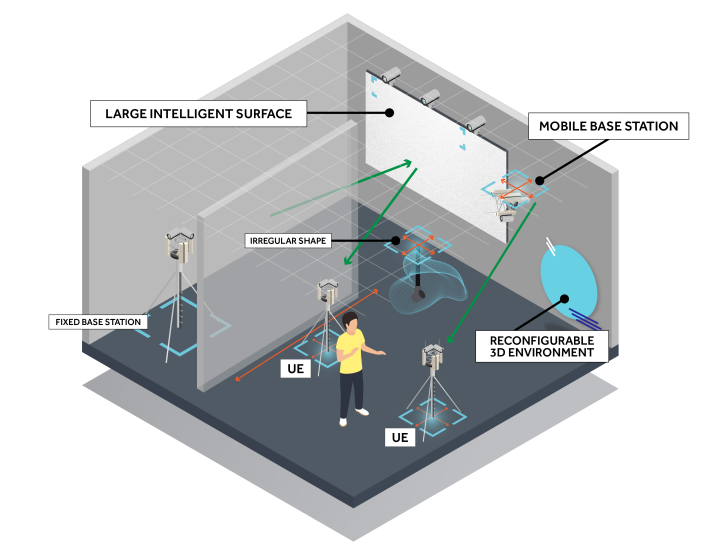
\includegraphics[width=0.7\linewidth]{figures/chamber_converge.png}
    \caption[Proposed vision-radio experimental chamber of the CONVERGE project]{Proposed vision-radio experimental chamber of the CONVERGE project \cite{converge2023_usecases}.}
    \label{fig:chamber_converge}
\end{figure}



Some of the questions mentioned in \cite{converge2023_usecases} to be addressed by the project are:

\begin{itemize}
    \item How to detect the location of obstacles to signal propagation, interfering terminals, and terminals served by the vision-aided mobile base station?
    \item How to jointly optimize beamforming, position, and traffic scheduling in the vision-aided mobile base station so that the Quality of Service offered to a set of terminals is maximized over time?
    \item How does incorporating visual information impact the Quality of Experience (QoE) for UEs in terms of throughput, latency, and reliability?
    \item Which machine learning techniques are better suited to enable dynamic, collaborative tracking by incorporating information from multiple base stations or cameras within a network under variable environmental conditions or UE behavior?
\end{itemize}

Given this scope, understanding the CONVERGE project’s architecture is required. It is
structured around three fundamental building blocks: the CONVERGE Chamber, the CONVERGE Core, and the CONVERGE Simulator, as illustrated in Figure \ref{fig:converge_arch}. This architectural division separates the physical infrastructure (the CONVERGE Chamber), the simulation infrastructure, the user interface, and the network and control functions, datasets,
and Machine Learning models (the CONVERGE Core).


\begin{figure}[H]
    \centering
    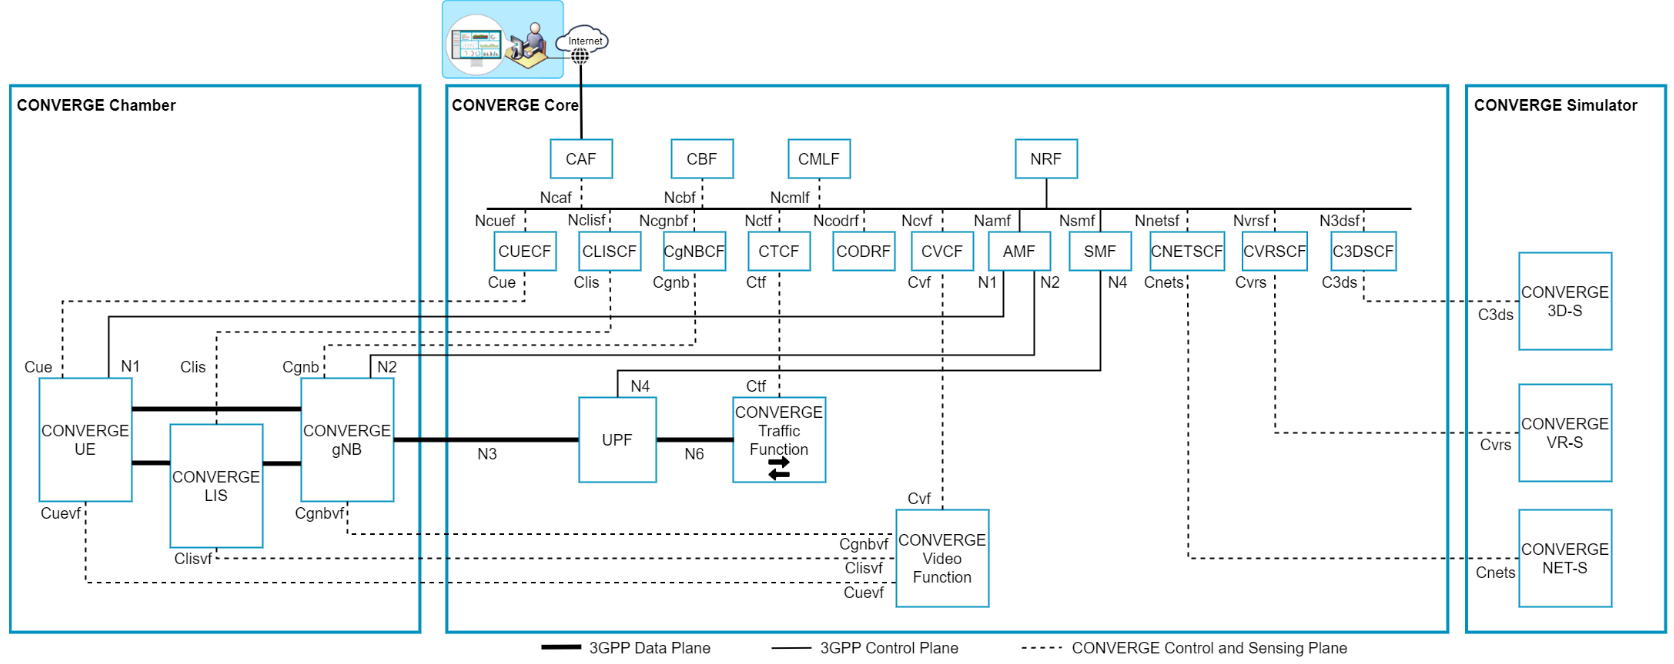
\includegraphics[width=1\linewidth]{figures/arch_converge.png}
    \caption[CONVERGE service-oriented architecture] {CONVERGE service-oriented architecture \cite{converge2023_specs}.}
    \label{fig:converge_arch}
\end{figure}

As detailed in \cite{converge2023_specs}, the CONVERGE Video Control Function (CVCF) is responsible for managing the video cameras facilitating the utilization
of video tools within the chamber. Moreover, it oversees and supports
vision models to extract information from the captured scenes. The CONVERGE Video Control Function collaborates with the CONVERGE gNB through the CONVERGE dedicated gNB Control Function (CgNBCF). This collaboration implies that the information from the video will be communicated to the CONVERGE gNB, enhancing its environmental awareness.
The CONVERGE Video Control Function, the gNB, and the Machine Learning models will
enhance connectivity and preemptively address challenges within the wireless environment.
By integrating advanced technologies and intelligent decision-making, the work
aims to contribute to the robustness and stability of wireless communications systems.


\section{Summary}\label{sec:Summary_SOA}
This chapter presents aspects of wireless communications, beginning with the evolution from 4G to 5G and the ambitious goals set for 6G. It also discusses the architecture of 5G, its components, and interfaces. Further, it presents approaches to Radio Access Network (RAN) deployment, such as cRAN, vRAN, and the Open-RAN (O-RAN) architecture.

A substantial portion focuses on describing CV tools and applications. It evaluates state-of-the-art detection and tracking models, focusing on the trade-off between speed, accuracy, and complexity. The discussion extends to open-source tools in CV, emphasizing their relevance to wireless communications challenges. The chapter also discusses the integration of CV into the broader context of wireless networks, providing a foundation for the subsequent exploration of video sensing in the field.

Additionally, the chapter presents related work to the problem posed in the introduction while presenting existing solutions leveraging video sensing. Finally, the CONVERGE project is presented since this dissertation will leverage the project's architecture. This chapter guides the current state of the convergence between CV and mobile networks, paving the way for a focused investigation in this dissertation.

% should i change the order of the sections?





    \chapter{System Specification, Design, and Implementation}\label{ch:specs_design_implem}

This chapter presents the proposed solution, including four main sections.
Section~\ref{sec:specs} discusses the requirements and specifications, Section~\ref{sec:prop_vision} presents the proposed vision module.
Section~\ref{sec:design} explains the solution design.
Finally, Section~\ref{sec:impl} presents the implementation of the system.

\section{System Specification}\label{sec:specs}
The goal of this dissertation was to extract vision-based information relevant to a 5G network.
This information should be available in near real-time to relevant entities of the network architecture upon subscription.
This solution envisions obstacle-aware networks and should enable a RAN to autonomously control the BS' placement and configuration based on the environment perception provided by the vision-based information.

\subsection{System Requirements}\label{subsec:system-requirements}

To demonstrate these concepts, we conceptualized a simple model.
The scenario is set in an indoor office environment, where it is determined if common objects will impact the LOS between a gNB and a UE\@.

To achieve this, specific system requirements were established to ensure the efficient detection, tracking, and dissemination of obstacles information within the 5G network.

The detailed requirements of the Computer Vision Module and its interface with the network are as follows:

\begin{enumerate}
    \item \textbf{Functional Requirements}
    \begin{enumerate}
        \item Detect and track objects in near real-time using computer vision algorithms.
        \item Identify specific obstacles and predict potential blockages.
        \item Send well-defined messages to a novel O-RAN xApp for further processing and decision-making.
        \item Ensure interoperability with the 5G network components via standardized messaging protocols. % should i use standarized, since there is no standard for it, i created a structure?
    \end{enumerate}
    \item \textbf{Non-Functional Requirements}
    \begin{enumerate}
        \item Maximize processing speed resorting to parallel processing on the GPU whenever possible\@.
        \item Minimize messaging latency ensuring rapid response by the xApp for optimal connection maintenance.
        \item High accuracy in object detection and tracking to minimize false positives and negatives.
        \item The solution should be scalable to handle multiple video streams, Base Stations, and UEs, allowing for broader deployment in various network environments.
        \item The system must use standardized messaging formats to ensure interoperability with different network components and vendors.
        \item The vision module and communications system should be robust, with mechanisms for error detection and recovery to maintain continuous operation.
        The model and its parameters are fundamental to assuring reliability. % how can i prove it?
    \end{enumerate}
\end{enumerate}

These requirements translate into Table ~\ref{tab:spec}, containing system specifications:

\begin{table}[H]
\caption{System Specifications.}
\label{tab:spec}
\centering
\resizebox{\textwidth}{!}{%
\begin{tabular}{|l|p{12cm}|}
\hline
\textbf{Specification} & \textbf{Description} \\ \hline
\textbf{Detection and tracking} & Use YOLOv5 Ultralytics \cite{ultralytics} and BoT-SORT \cite{botsort} for high accuracy and optimized speed. \\ \hline
\textbf{Messaging} & Encode messages using ASN.1 standards. \newline Transmit messages via SCTP protocol. \newline Include relevant information such as object ID, type, position ( cartesian coordinates), and confidence score. \\ \hline
\end{tabular}}
\end{table}

These specifications ensure that the Vision Module meets the requirements necessary for integration and operation within a 5G network environment.


Following these requirements and specifications, the system architecture was designed to facilitate efficient data processing.

\begin{figure}[H]
    \centering
    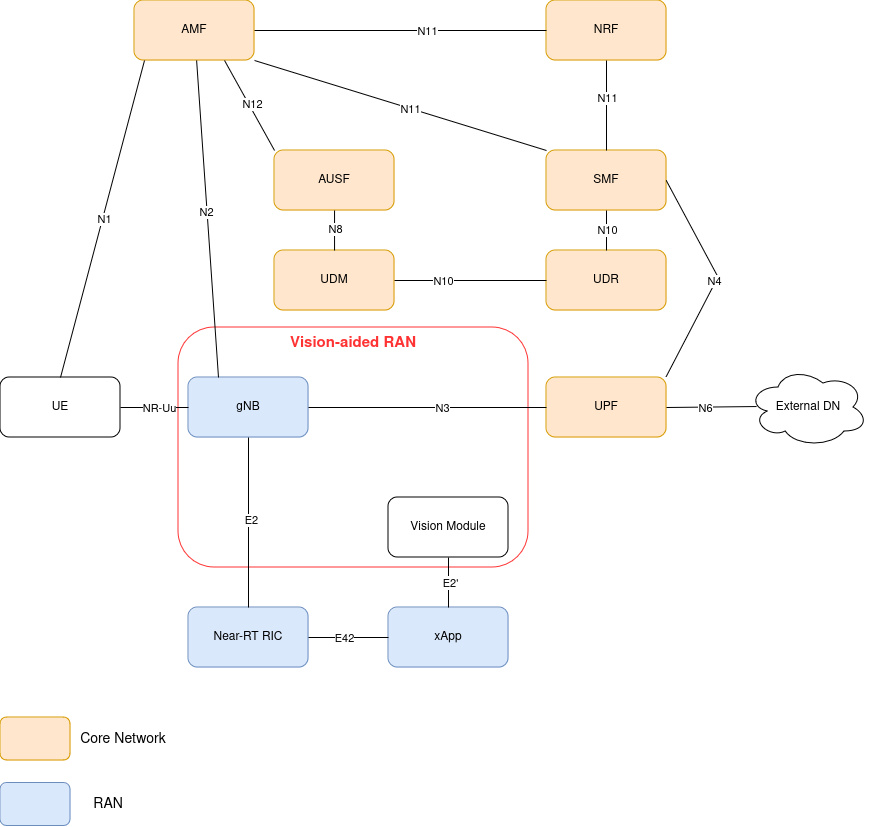
\includegraphics[width=0.7\linewidth]{figures/Syst_Arch.drawio}
    \caption[System Architecture of the proposed solution]{System Architecture of the proposed solution}
    \label{fig:my_arch}
\end{figure}

% draw: SMF[x], SPGWU[x], AMF[x], AUSF, UDM, UDR, mysql, NRF ext DN[x]
% requires improvements
In the proposed architecture, shown in Figure~\ref{fig:my_arch}, a UE requires 5G connectivity.
The 5G connection workflow begins with the UE initiating a connection request to the gNB, which then forwards the request to the AMF\@.
The gNB serves as the intermediary between the UE and the 5G core network, managing the radio resources, handling data transmission, and ensuring seamless connectivity as the UE moves.
The AMF authenticates the UE using credentials stored in the UDM. Upon successful authentication, the UE is granted access to the network.
The AMF and UPF then establish a data session for the UE, configuring the necessary resources for data transmission.
User data is transmitted between the UE and the UPF via the gNB\@.
The UPF routes the data to and from external networks, ensuring efficient data flow.

%------------ move to another place
%The 5G Core Network is responsible for managing the overall network functions, including authentication, mobility management, and routing of data.
%In our solution, both the RAN and the core are deployed within the same processing unit to maintain efficiency, mobility and simplicity.
%The AMF is a critical component of the 5G core that handles user authentication and mobility management.
%When a UE attempts to connect to the network, the AMF verifies the user's credentials and manages their session as they move across different cells in the network.

%The User Plane Function (UPF) manages the user data traffic, ensuring that data packets are efficiently routed between the UE and external data networks.
%It plays a pivotal role in delivering low-latency, high-bandwidth services to the end-users.
%Another essential core network function is the Unified Data Management (UDM), responsible for handling subscriber data and profiles.
%It ensures that user data is consistent and accessible across the network, supporting seamless user experiences.
%The User Plane Function (UPF) manages the user data traffic, ensuring that data packets are efficiently routed between the UE and external data networks.
%It plays a pivotal role in delivering low-latency, high-bandwidth services to the end-users.
%Another essential core network function is the Unified Data Management (UDM), responsible for handling subscriber data and profiles.
%It ensures that user data is consistent and accessible across the network, supporting seamless user experiences.

%To ensure the mobility and efficiency of our solution, the RAN and the core network components are deployed within the same processing unit.
%This integration offers several advantages.
%By colocating the RAN and core network functions, data processing and transmission delays are minimized, resulting in a more responsive network.
%The mobile RAN can seamlessly maintain connectivity with the UE, even when the gNB is moving, without relying on distant core network infrastructure.
%Having the RAN and core in a single unit simplifies the deployment process, making it easier to set up and manage the network in various locations, whether stationary or on the move.
%-------------------

In our solution, the RAN can be repositioned according to environment conditions that possibly affect the RF\@.
Those are reported by the Vision Module (Vision Module).
This enables the RAN to control manage its placement, based on those conditions together with radio metrics, such as SNR\@.
In order to establish the integration of Computer Vision into the 5G architecture, we took advantage of the Near-RT RIC, specified by O-RAN, to deploy a xApp responsible for the handling both radio metrics and the VM messages.
The communication between the VM and the xApp, is done through an interface inspired by the O-RAN E2 interface and E2 Application Protocol (E2AP).
This interface facilitates reliable data exchange using a SCTP socket connection (cf.Figure~\ref{fig:stack}) along with an Abstract Syntax Notation One (ASN.1) definition to structure the messages.
The use of ASN.1 ensures that the message formats are standardized, promoting interoperability and efficiency in data transmission.
This design allows the VM to communicate with the xApp, enabling the integration of data extracted from video for the mobile RAN management.

\begin{figure}[H]
    \centering
    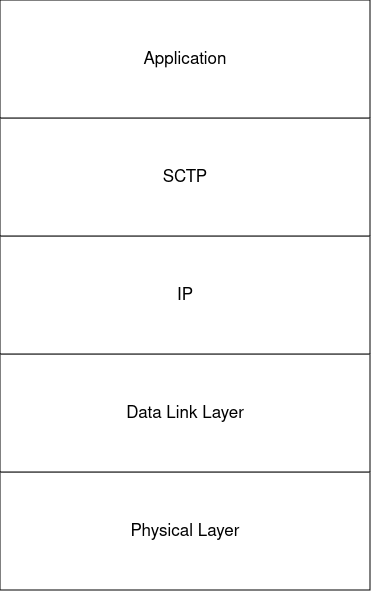
\includegraphics[width=0.35\linewidth]{figures/VisionModule_ProtocolStack.drawio(2)}
    \caption[Proposed Vision Module Protocol Stack]{Proposed vision module protocol stack.}
    \label{fig:stack}
\end{figure}


\section{Proposed Vision Module}\label{sec:prop_vision}
Our proposed vision module uses Computer Vision techniques to extract information about obstacles within the video camera's field of view.
This system processes video frames to detect and track obstacles, subsequently sending messages to services connected with relevant information.
The module sends five types of messages: blockage, future blockage, past blockage, the location of the UE and frame processed.
Table~\ref{tab:message_type} summarizes the description of each message type.
Each message will be explained further in the following sections.

\begin{table}[H]
    \caption{Summary of each message type}
    \label{tab:message_type}
    \centering
    \resizebox{\textwidth}{!}{%
        \begin{tabular}{|l|p{12cm}|}
            \hline
            \textbf{Type of message} & \textbf{Description} \\ \hline
            Blockage Messages & Sent when an obstacle is currently blocking the UE. \\ \hline
            Future Blockage Messages & Sent when an obstacle is predicted to block the UE based on its current trajectory. \\ \hline
            Past Blockage Messages & Sent when an obstacle that was previously blocking the UE is no longer doing so. \\ \hline
            UE Location Messages & Provide the current location of the UE. \\ \hline
            Frame Processed & Provide information that a frame of the video was processed. \\ \hline
        \end{tabular}}
\end{table}

The module includes functionality responsible for information exchange, detection and tracking, image processing, and utility functions.
We present a high level overview of the developed Vision Module.

The processing of the video starts with the capture of frames from the camera.
One frame is processed at a time.
The UE has a ArUco Marker in order to identify its placement.
OpenCV is responsible for identifying this marker and returning the ROI corresponding to the marker, as well as its identification.
Periodically, the Module sends a message containing the location (normalized cartesian coordinates) of the UE within the frame\@.
Following this, yolov8n, a YOLO pre-trained model jointly with BoT-SORT, is responsible for detecting and tracking the obstacles in the frame.
To improve control over frame selection for tracking detected objects, we have set specific parameters that allow timing adjustments in object detection.
This persistence has enabled us to extend the functionality of the Ultralytics API\@.

The main returned value by Ultralytics is a track history containing a unique identifier of the obstacle and its associated last positions (also normalized cartesian coordinates), alongside its classes and confidence scores.If it is noticed a difference between the last visible ArUcos and the current seen, the module checks if the obstacle last position intercepts the ArUcos position.
If this is true, the module generates a blockage message, indicating that an obstacle blocked the UE\@.
Immediately after the UE is unblocked, the module emits a message of Past Blockage, indicating that the LOS between gNB and UE returned.

Beyond that, the module is capable of predicting with certain anticipation that an obstacle seen by the camera will block the UE\@.
This is done using the tracking history constructed upon the results of the tracking.
This enables the calculation of the velocity of the objects.
Then, we can estimate the future positions and calculate whether the projected bounding boxes will intercept the ArUco.
This prediction allows us to reposition the gNB seeking the maintenance of the LOS and the channel quality assessed by the SNR\@.

The file \textit{ObstacleDetectionReport.asn} contains the specification of the set of messages created.
The messages are composed of a header and a payload.
The header of all messages is presented in Table~\ref{tab:header}:


\begin{table}[H]
    \caption{Components of the Message Header}
    \label{tab:header}
    \centering
    \resizebox{\textwidth}{!}{
        \begin{tabular}{|c|c|}
            \hline
            \textbf{Field} & \textbf{Description} \\ \hline
            messageType & Identifies the type of the message. \\ \hline
            timestamp & Identify the  timestamp in which the message was created. \\ \hline
            sourceId & Identify the source of the message.
            In this case, the Vision Module.\\ \hline
            destinationId & Identifies the intended recipient of the message.
            In this case, the xApp. \\ \hline
            e2InstanceId & Provides a unique identifier for the E2 interface instance associated with the message. \\ \hline
        \end{tabular}
    }
\end{table}

As for the content of the payload, it varies according to the type of message.
Each message requires different processing to extract the information required, as mentioned previously.
The following subsections present further each message type.

\subsection{Prediction of Blockage Messages}\label{subsec:prediction-of-blockage-messages}

To infer that an obstacle will block the line-of-sight (LOS) between the gNB and the UE, it is necessary to obtain a tracking history of the obstacle.
We achieved this by storing data over a number of frames, using the YOLO and BoT-SORT algorithms.
Once the tracking history is established, we have modeled the object's movement assuming a constant velocity.
This has proven effective for handling typical indoor movements, such as people walking or objects being moved.
By calculating the object's velocity, we can predict its future positions in upcoming video frames.
This allowed us to determine whether the obstacle will interrupt the LOS\@.
If the module predicts an impending blockage, it generates a message containing the information summarized in Table~\ref{tab:future_block_message}.


\begin{table}[H]
    \caption{Components of the Prediction of Blockage Payload}
    \label{tab:future_block_message}
    \centering
    \resizebox{\textwidth}{!}{
        \begin{tabular}{|c|c|}
            \hline
            \textbf{Field} & \textbf{Description} \\ \hline
            obstacleID & Unique identifier for the obstacle, provided by the tracking. \\ \hline
            obstacleType & Type of the obstacle detected. \\ \hline
            obstacleLocation & Location of the detected obstacle within the frame ( normalized cartesian coordinates). \\ \hline
            obstacleVelocity & Velocity of the detected obstacle (normalized vector). \\ \hline
            obstacleConfidence & Confidence level in the identification of the object. \\ \hline
            timeToCross & Predicted time  that the obstacle will obstruct the UE. \\ \hline
            ueId & Identifier for the UE, in this case its ArUco identifier. \\ \hline
        \end{tabular}
    }
\end{table}




\subsection{Blocking messages}\label{subsec:blocking-messages}

In order to indicate that an obstacle is blocking the LOS between gNB and UE, it is
\textcolor{red}{Continue}

\begin{table}[H]
    \caption{Components of the Prediction of Blockage Payload}
    \label{tab:block_payload}
    \centering
    \resizebox{\textwidth}{!}{
        \begin{tabular}{|c|c|}
            \hline
            \textbf{Field} & \textbf{Description} \\ \hline
            obstacleID & Unique identifier for the obstacle, provided by the tracking. \\ \hline
            obstacleType & Type of the obstacle detected. \\ \hline
            obstacleLocation & Location of the detected obstacle (x,y normalized coordinates, in the frame). \\ \hline
            obstacleConfidence & Confidence level in the identification of the object. \\ \hline
            timeBlocked & Time the obstacle has been blocking, up to 5000 milliseconds (optional). \\ \hline
            ueId & Identifier for the UE, in this case its ArUco identifier. \\ \hline
        \end{tabular}
    }
\end{table}


\subsection{Past Blockage}\label{subsec:past-blockage}

This message is sent to inform that the UE is no longer blocked by the obstacle.
Table~\ref{tab:past_block_payload} presents the fields for the
\textcolor{red}{Continue}

\begin{table}[H]
    \caption{Components of the payload of PastBlockage Message}
    \label{tab:past_block_payload}
    \centering
    \resizebox{\textwidth}{!}{
        \begin{tabular}{|c|c|}
            \hline
            \textbf{Field} & \textbf{Description} \\ \hline
            obstacleID & Unique identifier for the obstacle, provided by the tracking. \\ \hline
            obstacleType & Type of the obstacle detected. \\ \hline
            obstacleLocation & Location of the detected obstacle (x,y normalized coordinates, in the frame). \\ \hline
            obstacleConfidence & Confidence level in the identification of the object. \\ \hline
            ueId & Identifier for the UE, in this case its ArUco identifier. \\ \hline
        \end{tabular}
    }
\end{table}


\subsection{Location of UEs}\label{subsec:location-of-ues}
The message presents the location data of the UEs. Table~\ref{tab:ue_payload} presents the message payload.
To extract this information, it is necessary to detect the bounding boxes of the markers associated with the UEs.
The system continuously monitors the movement of the UEs and transmits updates whenever changes are detected.
This process involves identifying and tracking the bounding boxes of the ArUco markers associated with the UEs.
Then, comparing the current visible ArUco IDs with the previously detected IDs. This is done though buffering, temporarily storing changes to ensure accuracy and consistency.
Periodically, location reports are sent when changes in the UEs' positions are confirmed.
This approach ensures precise and timely updates on the UEs' locations.

\begin{table}[H]
    \caption{Components of the UE Location Message payload}
    \label{tab:ue_payload}
    \centering
    \resizebox{0.7\textwidth}{!}{
        \begin{tabular}{|c|c|}
            \hline
            \textbf{Field} & \textbf{Description} \\ \hline
            ueLocation & Contains the location of the UE. \\ \hline
            ueId & Identifier for the UE, based on the ArUco ID. \\ \hline
        \end{tabular}
    }
\end{table}




\subsection{Frame Processed}\label{subsec:frame-processed}
In our system, frame processed messages play an important role in maintaining communication and monitoring the performance of the Vision Module.
These messages are primarily designed to inform the xApp that the Vision Module is actively running and processing frames.
Additionally, they allow for the tracking of the time taken to process each frame, which is essential for performance optimization and debugging purposes.

The frame processed message contains the following fields, as detailed in Table~\ref{tab:frame_proc_pay}:

\begin{table}[H]
    \caption{Components of the Frame Processed Message payload}
    \label{tab:frame_proc_pay}
    \centering
    \resizebox{0.7\textwidth}{!}{
        \begin{tabular}{|c|c|}
            \hline
            \textbf{Field} & \textbf{Description} \\ \hline
            frameID & Sequential identification number of the frame \\ \hline
            timeProcessed & Time taken to process the frame in milliseconds \\ \hline
        \end{tabular}
    }
\end{table}

These messages serve as heartbeat signals to the xApp, confirming the Vision Module's operational status and performance.
By continuously sending frame processed messages, the system ensures that the xApp is kept up-to-date with the Vision Module's activity.


\section{System Design}\label{sec:design}

This section presents the system designed to implement and evaluate the proposed solution.
The system is depicted in Figure~\ref{fig:design_arch}.
It is composed of two main logical units.
The first implements the 5G Core Network, the Near-RT RIC and the Vision-aided gNB\@.
The second unit implements the UE software.


\begin{figure}[H]
    \centering
    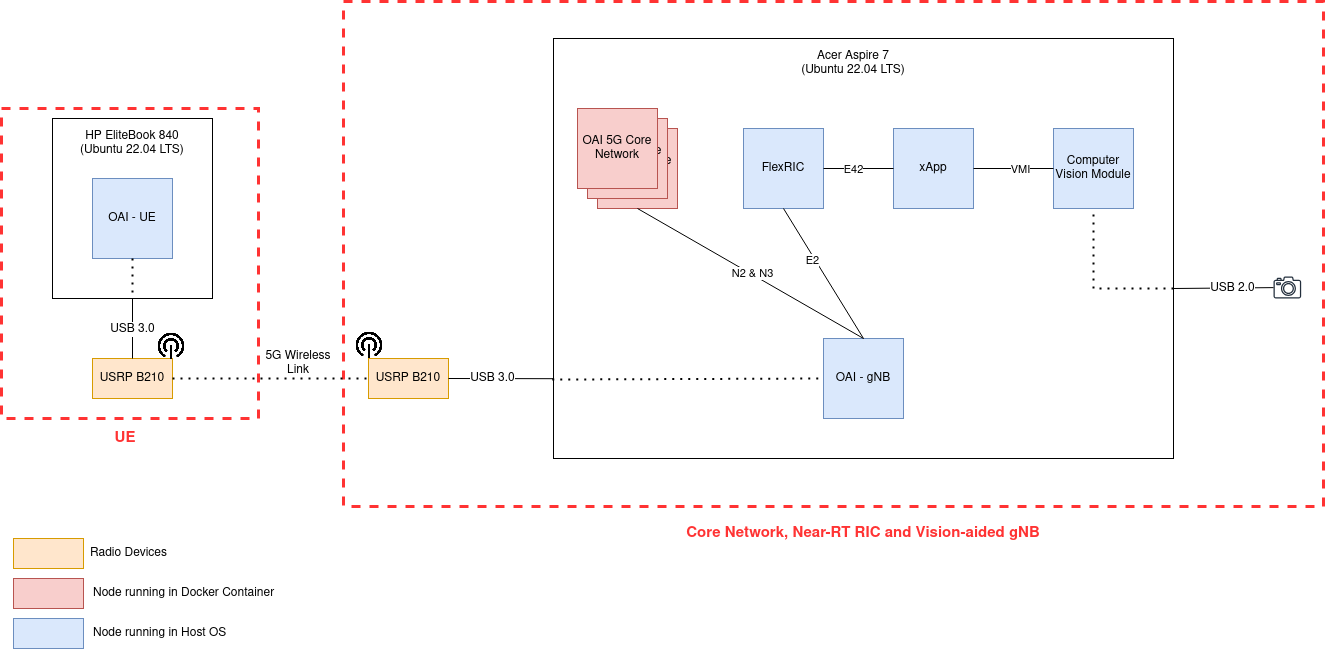
\includegraphics[width=0.7\linewidth]{figures/System Arch.drawio}
    \caption[System architecture designed for implementing and evaluating the proposed solution]{System architecture designed for implementing and evaluating the proposed solution.}
    \label{fig:design_arch}
\end{figure}

The following subsections detail the hardware used in the implementation and the choices for software packages.


\subsection{Software}\label{subsec:software}
This section presents the main software packages used to develop the Vision Module and implement the 5G network.
Beyond this, in the repository containing the VM, there is a file for reproducing the Python virtual environment.

\subsubsection{OpenCV}
% revision
There are several open-source software packages available for Computer Vision in Python.
Open Source Computer Vision Library (OpenCV) is one of them.
It contains several optimized algorithms, which can be used for different tasks, including object detection, image processing, and real-time video analysis.
This diverse support makes it suitable for both basic tasks and complex applications requiring advanced functionalities.
Moreover, OpenCV's well-documented API facilitates ease of use and integration into various projects, ensuring efficient development and deployment.
Unlike some other libraries that may focus on specific aspects of image processing or lack support across different domains, OpenCV provides a solution with cross-platform compatibility, making it applicable across diverse operating systems and hardware setups.
Furthermore, OpenCV benefits from a large and active community, offering extensive resources, tutorials, and community support, which are invaluable for developers and researchers seeking assistance or collaboration in tackling complex computer vision challenges effectively and efficiently.
Therefore, OpenCV is the leading choice for robust and scalable computer vision applications.

Additionally, OpenCV is the only library who directly supports ArUco Markers.
ArUco is a widely-used open-source library for Augmented Reality (AR) applications that involves detecting and tracking augmented markers.
These markers are specially designed square or rectangular patterns with a unique binary encoding, which can be printed and placed in the physical environment.
ArUco markers are typically used in computer vision tasks to provide reference points in a scene, enabling accurate localization and tracking of objects or video cameras.

OpenCV emerges as the premier choice among general computer vision libraries, distinguished by its extensive feature set, optimized performance, and robust community support.
Unlike scikit-image \cite{}, which excels in image processing tasks with functions for filtering, morphology, and segmentation, OpenCV offers a broader range of over 2500 optimized algorithms spanning image and video processing, object detection, and video camera calibration.
In contrast to Pillow (PIL Fork) \cite{}, which specializes in image format handling and basic manipulation, OpenCV provides comprehensive tools for both foundational and advanced computer vision applications.
Moreover, while SimpleCV \cite{} simplifies OpenCV usage with a user-friendly interface, OpenCV's C++ backend and GPU acceleration capabilities enable superior performance, which is crucial for real-time processing and large-scale data operations.

In our proposed solution, OpenCV is utilized to:
\begin{itemize}
    \item \textbf{Obtain Frames:} OpenCV is used to capture video frames from the video camera.
    It provides easy-to-use interfaces to capture and manipulate video streams from various input sources.
    \item \textbf{Detect ArUco Markers:} OpenCV includes modules for detecting ArUco markers, which are widely used in computer vision applications for video camera calibration, pose estimation, and augmented reality.
    In our solution, these markers help in identifying the UEs without the need to train the YOLO model to perceive such objects.
\end{itemize}

\subsubsection{Ultralytics YOLO}
As discussed in Section ~\ref{sec:CV}, Ultralytics YOLO (You Only Look Once) is a state-of-the-art, real-time object detection solution.
It is known for its speed and accuracy, making it suitable for applications that require fast and reliable object detection and tracking.
While there are other solutions, also preseted in that Section, we chose Ultralytics YOLO due to simplicity, integration and since it is suitable for the intended application and use in state-of-the-art object detection and tracking situations.

In our proposed solution, Ultralytics YOLO is employed to:
\begin{itemize}
    \item \textbf{Detection:} YOLO is used to detect various objects in the frames captured by the video camera.
    Its real-time capabilities allow for the immediate identification of obstacles within the field of view.
    \item \textbf{Tracking:} YOLO’s tracking module is used to keep track of detected objects over successive frames.
    This is crucial for maintaining the continuity of object identification and for predicting future positions of the obstacles. %BOTSORT and BYTETRACK
\end{itemize}

The combination of OpenCV and Ultralytics YOLO allows for robust detection, tracking, and message exchange functionalities in our vision module.
OpenCV handles the initial capture and processing of video frames, while YOLO and BoT-SORT performs the real-time detection and tracking of objects.
This integrated approach ensures that the vision module can effectively monitor and report on obstacles, providing key information to subscribed services.

\textcolor{red}{CITATIONS}
\subsubsection{ASN1Tools and ASN1C}
There are a few open-source libraries available for handling ASN.1.
FlexRIC utilizes asn1c~\cite{}, so for simplicity we chose the same for the xApp (client).
asn1c~\cite[asn1c]{} is a open-source ASN.1 compiler that generated C/C++ code for ASN.1 data structures, supporting different encoding rules.
While this library also supports Python, we chose not to use it, since there are simpler APIs specially tailored for Python development.
As for the Vision Module (Python server), we chose ASN1Tools because it offers certain advantages.

ASN1Tools is a Python library provides a simple way to handle ASN.1 data structures, through a straightforward API\@.
The library support for a range of ASN.1 specifications and encoding rules, including BER, DER, and PER\@.
Moreover, ASN1Tools is actively maintained, with regular updates and improvements.
This guarantees that we have access to the latest features and bug fixes, which enhances the reliability and stability of our system.
ASN1Tools is optimized for performance, allowing for fast encoding and decoding operations.
This optimization is suited for real-time applications like our Vision Module, where processing speed is essential to maintain system responsiveness and accuracy.

While other libraries such as pyasn1 and libasn1 are available, they have certain limitations.
pyasn1, for instance, is less efficient in terms of performance and has a more complex API\@.
libasn1, part of the GNU project, is less user-friendly and optimized for performance.

\textcolor{red}{CITATIONS}
\subsubsection{5G Core Network, 5G gNB, and 5G UE}
The main open-source 5G software packages for implementing an O-RAN based architecture are OAI~\cite[]{} and srsRAN~\cite{}.
For our system, we chose OAI because it provides all the necessary components to deploy a 5G standalone network, including both the RAN and Core network.
In contrast, srsRAN only supports the deployment of the RAN, requiring an additional software package, such as OAI, to implement the Core network.

\subsubsection{Near-RT RIC}
The main open-source software packages able to implement a Near-RT RIC are Mosaic5G’s FlexRIC~\cite[]{} and  O-RAN Software Community’s Near-RT RIC~\cite[]{}.
FlexRIC was chosen for our solution due to its lightweight nature, launched from an executable file.
\textcolor{red}{Include disadvantage of ORAN RIC}

\subsection{Hardware}\label{subsec:hardware}

\textcolor{red}{CITATIONS}
\subsubsection{Core Network, FlexRIC, Computer Vision module and gNB}
The OAI Core Network, FlexRIC,the Computer Vision module and the gNB were deployed in a laptop Acer Aspire A715-74G\@.
The OAI Core was deployed using Docker containers, requiring 4 cores CPU, 16GB of RAM and a minimum of 1.5GB free storage for the docker images.
As for FlexRIC, it does not have hardware requirements listed, but while deploying it was noticed that it is not resource intensive, sufficing the same ones required for the Core Network.
The xApp was deployed alongside FlexRIC in order to assure reduced latency between the two components.
Also,  the way interface E42 is implemented requires them to be running in the same computing unit.
As for the gNB, the hardware recommended are 8 physical CPU cores and 32 GB of RAM\@.
While the laptop used did not fulfill these requirements, it has proven sufficient to run the OAI gNB software, as it was noted before in~\ref{}. % ref to dissertation of gonçalo

As for the Computer Vision Module, the minimal hardware requirement is a CUDA-compatible GPU ~\cite{}, for Ultralytics YOLO model to properly run.
Given that for our solution pre-trained model has proven enough to accurately detect and track objects, we did not worried about fulfilling the

\textcolor{red}{FINALIZE}



Table ~\ref{tab:specs_pc} presents the specification of the computer.

\begin{table}[H]
    \begin{tabular}{|c|c|}
        \hline
        \textbf{Specification} & \textbf{Details} \\ \hline
        Processor                      &           Intel(R) Core(TM) i5-9300H CPU @ 2.40GHz   \\ \hline
        RAM                      &          16GB        \\ \hline
        Disk                      &   2 SSDs  512GB and 256GB         \\ \hline
        GPU                     &   GeForce GTX 1050 (3GB)      \\ \hline
        Operational System & Ubuntu 22.04.4 LTS                  \\ \hline
    \end{tabular}\label{tab:specs_pc}
\end{table}

For the Computer Vision Module, we opted to use a webcam due to its simplicity and ease of integration.
The chosen webcam, a model LL-4196, offers Full HD (1920 x 1080 Pixels) resolution and supports a frame rate of 30 FPS\@.
This ensures that the video feed acquired is of high quality, providing sufficient detail and smooth motion necessary for accurate computer vision processing.
The camera connects to the computer using a USB 2.0 interface.
The specifications of the camera are sufficient for the system to detect and track movements and objects within the environment, assuring the efficient operation of the Computer Vision Module.
% why? velocity constant , processing of frame
\textcolor{red}{Mention the comparision between dispacement of objects and processing rate}

Deploying the gNB and the UE in two different host computers implicates the use of Software-Defined Radio (SDR) in order to establish a 5G connection between the gNB and the UE.
OAI recommends the use of three SDR models: USRP B210, USRP N300 and USRP X300\@ \cite{}. %https://gitlab.eurecom.fr/oai/openairinterface5g/-/blob/develop/doc/NR_SA_Tutorial_OAI_nrUE.md
For our implementation, we have selected the first since it is cost-effective and a popularity across the community.
This model uses a USB 3.0 interface to connect to the computer acting as a processing unit.
The SDR was equipped with two W5208K dipole antennas.
Figure~\ref{fig:SDRs} shows the two SDRs with their respective antennas.
We have selected 3.6GHz as the carrier frequency for the 5G RAN\@.

\begin{figure}[H]
    \centering
    
\includegraphics[width=0.7\linewidth]{figures/uporto-feup}
    \caption{SDRS}
    \label{fig:SDRs}
\end{figure}



\subsubsection{UE}
The UE was deployed in HP EliteBook 840 Laptop.
The hardware requirements for the deployment of the UE are 8 cores and 8GB of RAM\@.
Table~\ref{tab:specs_pc_ue} depicts the specification of the computer responsible for the UE\@.

\begin{table}[H]
    \begin{tabular}{|c|c|}
        \hline
        \textbf{Specification} & \textbf{Details} \\ \hline
        Processor                      &  Intel(R) Core(TM) i7-5600U CPU @ 2.60GHz          \\ \hline
        RAM                      &          16GB        \\ \hline
        Disk                      &   128GB         \\ \hline
        GPU                     &   Intel Corporation HD Graphics 5500                \\ \hline
        Operational System & Ubuntu 22.04.4 LTS                  \\ \hline  %  check
    \end{tabular}\label{tab:specs_pc_ue}
\end{table}

\section{System Implementation}\label{sec:impl}
For the Vision Module:

    Coding:
        Implementing object detection and tracking using YOLO and BoT-SORT algorithms.
        Implementing ArUco marker detection using OpenCV
        Developing the communication interface using SCTP and ASN.1 for message encoding.
        Handle video input, process each frame, and generate output messages.

    Testing:
        Running unit tests to ensure each component (detection, tracking, messaging) works as intended.
        Conducting integration tests to verify that components interact correctly.
        Performing system tests with both pre-recorded videos and real-time captures to ensure the module meets the specified performance criteria (e.g., processing speed, accuracy).

    Deployment:
        Deploying the vision module on the specified hardware.
        Monitoring performance in real-time scenarios to ensure it meets the defined requirements.
        Making adjustments and optimizations based on observed performance and feedback.

\textcolor{red}{adjust hole vision module part}
The module includes functions responsible for communication, detection and tracking, image processing, and utility functions.
We present a high level functionality overview of the developed Vision Module.
We utilized multi-threading in order to assure the timely processing of the video.
The first thread is responsible for handling communication, i.e.\ the connection with the xApp and sending the generated messages.
The second thread is responsible for the video processing, i.e.\ identifying objects and generating messages corresponding to the environment perception.

The processing of the video starts with the capture of frames from the camera.
One frame is processed at a time.
The UE has a ArUco Marker in order to identify its placement.

Arquitetura cliente servidor
Como integrar e testar - multi-threading  --comm e processing video.

\textcolor{red}{CITATIONS}
\subsection{OAI 5G Core Network}\label{subsec:oai-5g-core-network}
OAI offers three methods for implementing the Core Network: bare-metal installation or virtual machines, automated deployment of network functions (NFs) in Docker containers using Docker-Compose, and cloud-native deployment using Helm Chart on OpenShift or Kubernetes clusters ~\cite{}.
Choosing Docker for deployment simplifies the process by encapsulating network functions in containers, making them easier to manage, scale, and automate, which enhances the overall efficiency and flexibility of the network infrastructure.

Besides that, the Core can be implemented in two scenarios.
We chose scenario I , since it contains the minimum components necessary in order to test end to end connectivity between the nodes.
This scenario contains 8 containers.
python3 core-network.py --type start-basic --scenario 1
- Scenario I:  AMF, SMF, UPF (SPGWU), NRF, UDM, UDR, AUSF, MYSQL

\textcolor{red}{Finish explanation}

\textcolor{red}{CITATIONS}
\subsection{OAI gNB}\label{subsec:oai-gnb}
The deployment of the OAI gNB, we used the latest version of OAI RAN. In order to deploy the gNB with the SDR, it was required to do some alterations to \textit{gnb.sa.band78
.fr1.106PRB.usrpb210.conf} configuration file.
Namely, edit MCC, MNC and TAC values to assure they corresponded to the values present in the Core \textit{docker-compose.yaml} file.
If these values do not align, the NGAP setup between AMF and gNB over N2 interface will fail.
It is also necessary to modify the IP address of the AMF and an IP so that the gNB can communicate with the AMF and SMF\@.

\textcolor{red}{CONTINUE}

Finally, it is necessary to establish a connection between the OAI gNB software and the SDR\@.
As recommended by OAI, we utilized the USRP Hardware Driver (UHD)~\cite{}.
UHD is a driver that enables communication between software and USRP hardware, providing a standardized interface for configuring and controlling aspects of the SDR devices, such as frequency, sample rate, gain, and antenna settings.
Figure~\ref{fig:uhd_probe} illustrates the UHD driver detecting the USRP device, loading its firmware, and performing diagnostic tests.

\begin{figure}[H]
    \centering
    
\includegraphics[width=0.7\linewidth]{figures/uporto-feup}
    \caption{UHD obtaining information about the connected USRP device and testing it}
    \label{fig:uhd_probe}
\end{figure}

\subsection{OAI 5G UE}\label{subsec:oai-5g-ue}
In order to deploy the OAI UE, we needed to initiate the OAI UE software modem with parameters corresponding to the gNB settings.
The command used is as follows:

\lstinline[columns=flexible,breaklines=true]{sudo ./nr-uesoftmodem -r 106 --numerology 1 --band 78 -C 3619200000 --ue-fo-compensation --sa -E --uicc0.imsi 208990200000001}


The parameters are:

\begin{itemize}
    \item \texttt{-r 106}: Sets the radio configuration to 106.
    This must match the radio configuration set on the gNB to ensure proper communication.
    \item \texttt{--numerology 1}: Specifies the numerology index, set to 1, defining sub carrier spacing and slot duration.
    The gNB must use the same numerology index for compatibility.
    \item \texttt{--band 78}: Configures the UE to operate in the n78 band.
    The gNB is also set to operate in the n78 band, facilitating the connection.
    \item \texttt{-C 3619200000}: Sets the center frequency to 3619.2 MHz. The gNB is configured to transmit on this same center frequency.
    \item \texttt{--ue-fo-compensation}: Enables frequency offset compensation for the UE, ensuring synchronization with the gNB.
    \item \texttt{--sa}: Indicates that the UE is operating in standalone mode, directly connecting to the 5G network without relying on an LTE anchor, matching the gNB configuration.
    \item \texttt{-E}: Specifies that the program should utilize 75\% of the sampling rate frequency.
    \item \texttt{--uicc0.imsi 208990200000001}: Sets the IMSI for the UE to \texttt{208990200000001}.
\end{itemize}

We needed to use one of the International Mobile Subscriber Identity (IMSI) values present in the Core database to ensure that the UE could authenticate successfully.
The IMSI value, \texttt{208990200000001}, was selected from the Core database and used in the \texttt{nr-uesoftmodem} command.
This selection was crucial because it aligns with the subscriber information stored in the network, facilitating proper authentication and allowing the UE to connect and communicate with the network.
By ensuring that the IMSI used in the UE configuration matches an entry in the Core database, we verify that the UE can be authenticated correctly and allowed access to the network services.

If we use an IMSI value that is not present in the Core database, the authentication process will fail, as illustrated by the Wireshark capture shown in Figure~\ref{fig:UE_failure}.

\begin{figure}[H]
    \centering
    
\includegraphics[width=0.7\linewidth]{figures/uporto-feup}
    \caption{UE registration rejected due to UE SIM details}
    \label{fig:UE_failure}
\end{figure}

\subsection{FlexRIC}\label{subsec:flexric}
FlexRIC is deployed in the same computer as the OAI 5G Core Network.
The procedure is to install the required dependencies and compile FlexRIC software.
By default, FlexRIC is configured to run on the Loopback Interface address (127.0.0.1).
Since we are deploying gNB and FlexRIC in the same Host, this is not necessary to change.
In order to assure the use of the E2 Agent, is necessary to include in the configuration file of the gNB the following:

\begin{verbatim}
e2_agent = {
  near_ric_ip_addr = "127.0.0.1";
  sm_dir = "/usr/local/lib/flexric/"
}
\end{verbatim}

This informs that FlexRIC is running on the localhost IP, indicating that the RIC is running on the same machine as the E2 agent.
The directory informs where the Service Models for FlexRIC are located.
This is essential to assure the correct communication between OAI gNB and FlexRIC\@.



\section{Summary}\label{sec:summary}
Our proposed architecture is divided into two logical units.
The first one comprises the OAI 5G Core Network, FlexRIC, xApp and Vision Module, deployed in an Acer Aspire Laptop.
The second unit comprehends the OAI UE, deployed in an HP Elitebook.
The gNB and the UE used USRP B210 SDR board to connect via 5G Wireless Link.
The Vision Module received a video feed, processed it and sent relevant obstacle information seen in the video, via its interface.
The xApp was responsible for monitoring the received messages and the SNR.
The chapter demonstrates the feasibility and benefits of integrating computer vision with mobile communications.
By leveraging Computer Vision, the quality of the communication channel can be enhanced.







    \chapter{System Validation}\label{ch:validation}

\textcolor{red}{THIS IS AN UNFINISHED CHAPTER}

This chapter presents the validation of the proposed solution.
The validation process is described into different sections, each addressing different components of the system.
Section~\ref{sec:meth} outlines the methodology used for validation.
Section ~\ref{sec:experimental-setup} presents the experimental setup.
In Section ~\ref{sec:component-testing}, each component is tested.
\textcolor{red}{UPDATE ACCORDINLY}
Section~\ref{sec:use_case} presents a specific use case to demonstrate the system's functionality.
Finally, Section~\ref{sec:discuss} provides a discussion of the results and insights gained from the validation process.

\section{Methodology}\label{sec:meth}
We have divided our tests into three categories: Component Testing, Interoperability Testing and Use Case Validation.
The first was used to validate the proper functioning of each component, with a performance evaluation when possible.
The second category serve to determine if the components were working jointly properly.
The last seek to validate the proposed system in a reference scenario.
In each set of tests, we conducted a functional validation using tools such as ping and Iperf.
When applicable, the performance was evaluated.
\textcolor{red}{Maybe write something more}

\section{Experimental Setup}\label{sec:experimental-setup}
This section presents the experimental setup.
Figure~\ref{fig:setup} shows a photograph of the experimental scenario.

\begin{figure}[H]
    \centering
    
\includegraphics[width=0.5\linewidth]{figures/uporto-feup}
    \caption{Experimental setup}
    \label{fig:setup}
\end{figure}


\section{Component testing}\label{sec:component-testing}


\subsection{Core Network}\label{subsec:core_network}
In this section, the Core Network configuration and validation are discussed.
It includes the setup of network elements, their interactions, and performance metrics.
In order to make sure that all Core Network components are working properly, we performed a test.
The deployment of the Core Network is done through Docker containers.
Figure~\ref{fig:core_init} presents the command for running the Core Network setup script.
After the initialization of the Docker containers, it is possible to see the logs of the setup script, indicating the successful initialization.

\begin{figure}[H]
    \centering
    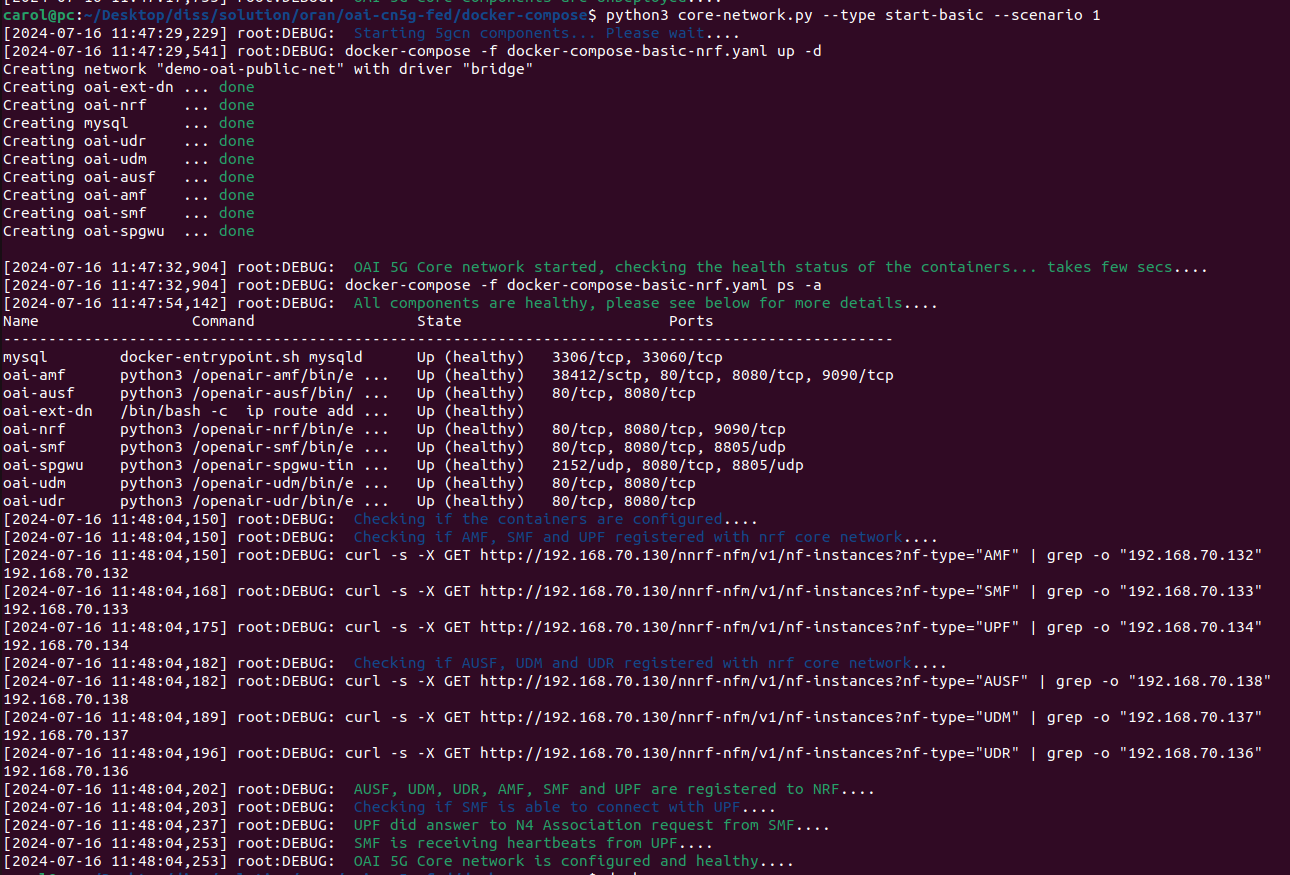
\includegraphics[width=0.5\linewidth]{figures/core_init}
    \caption[Initialization of the Core Network]{Initialization of the Core Network}
    \label{fig:core_init}
\end{figure}

In order to confirm the correct deployment, the interface \textit{demo-oai} must appear when running the \textit{ifconfig} command.

Then, we verified that all the containers had connectivity using the interface created in the Host OS, using the ping tool,as shown by Figure~\ref{fig:ping_core}.
Each interface sends requests to each network component according to the table~\ref{tab:ip_core}.

\begin{figure}[H]
\centering

\includegraphics[width=0.5\linewidth]{figures/uporto-feup}
\caption[Pinging NRF, MySQL Database, AMF, SMF, UPF, UDR, UDM and AUSF respectively from Host OS
interface]{Pinging NRF, MySQL Database, AMF, SMF, UPF, UDR, UDM and AUSF respectively from Host OS
interface}
\label{fig:ping_core}
\end{figure}


Successfully concluding this tests ensures that the 5G Core Network is operational.

\section{FleXRIC}\label{sec:flexric}
As for the FlexRIC deployment, it is simply necessary to assure its correct launch.
Upon launching, it awaits for incoming connection requests from an E2 Node.
Figure~\ref{fig:near-rt-ric} shows the initialization of the FlexRIC\@.

\begin{figure}[H]
    \centering
    
\includegraphics[width=0.5\linewidth]{figures/uporto-feup}
    \caption{Initialization of FlexRIC's executable}
    \label{fig:near-rt-ric}
\end{figure}

When it is properly launched, the gNB can be initialized.

\section{gNB}\label{sec:gnb}
\textcolor{red}{Finish}
To ensure the correct functioning of the gNB, it should be registered in the 5G Core Network, connected to the FlexRIC and registered as a E2 node.
They need to be validated separately since the connections are independent.

To access the gNB connectivity to the Core, we need to check the connection between the gNB Host and the AMF and UPF, since the gNB needs to communicate with them.
This can be tested with ping from the gNB's Host to these entities.
Figure~\ref{fig:ping_gnb} shows the results.

% figure with ping to AMF and UPF 132 and 134

\begin{figure}[H]
    \centering
    
\includegraphics[width=0.5\linewidth]{figures/uporto-feup}
    \caption{Conection test to AMF and UPF, respectively, from gNB Host.}
    \label{fig:ping_gnb}
\end{figure}

After

\section{UE}\label{sec:ue}
\textcolor{red}{Finish}

In order to test the correct initialization of the UE we needed to ensure connection with the Core Network.
After executing the command present in~\ref{subsec:oai-5g-ue}, we observed in Wireshark the correct registration of the UE in Figure~\ref{fig:registration_ue}.

\begin{figure}[H]
    \centering
    
\includegraphics[width=0.5\linewidth]{figures/uporto-feup}
    \caption{Registration of the UE}
    \label{fig:registration_ue}
\end{figure}

When this synchronization occurs, we can verify the creation of \textit{oaitun\_ue1}, the tunnel interface between UE and Core Network.
With that, we can test its connectivity, by pinging to every Core Network component, as well as the Internet.
Figures~\ref{fig:ping_ue_core} and~\ref{fig:ping_ue_internet} shows the outcome of these tests, to Core and to the Internet respectively.

\begin{figure}[H]
    \centering
    
\includegraphics[width=0.5\linewidth]{figures/uporto-feup}
    \caption{Pinging from UE to the Core Components}
    \label{fig:ping_ue_core}
\end{figure}

\begin{figure}[H]
    \centering
    
\includegraphics[width=0.5\linewidth]{figures/uporto-feup}
    \caption{Pinging from UE to Google's public DNS server}
    \label{fig:ping_ue_internet}
\end{figure}




\section{Computer Vision Module}\label{sec:cv_module}
To ensure the correctness and reliability of the computer vision module, a series of validation tests were conducted.
These tests were designed to evaluate both the processing capabilities of the module and the accuracy of the message exchange between the vision module and the xApp.

The processing time of each frame was measured to assess the real-time performance of the computer vision module.
This is important to ensure that the module could keep up with dynamic environments, such as an office setting where people and objects are constantly moving.
The tests showed that the processing times were within acceptable limits, allowing for timely detection and response.
% show some math on why this result is sufficient
% plot some results

A reference video was used to evaluate the detection and tracking results of the computer vision module.
This video, containing typical office movements like people walking and objects being moved, was processed to check for detection accuracy and tracking consistency.
The results confirmed that the module could accurately detect and track objects, validating its effectiveness in a real-world scenario.
Figure~\ref{fig:reference_video} shows the

% image of a frame of the video and the corresponding messages
\begin{figure}[H]
    \centering
    
\includegraphics[width=0.5\linewidth]{figures/uporto-feup}
    \caption{Reference video and corresponding messages generated.}
    \label{fig:reference_video}
\end{figure}

Print statements were used on the server side to verify the correct formatting, coding, and decoding of the messages.
This step was crucial to ensure that the messages sent from the computer vision module to the xApp were correctly structured and could be properly interpreted upon receipt.

On the client side,the xApp, print statements were employed to confirm the correct reception of the messages.
This validation step ensured that the messages transmitted through the socket connection were received intact and could be  correctly processed.

To further validate the communication, Wireshark was used to capture SCTP packets containing the messages exchanged between the server and client.
This capture provided a detailed view of the message flow, confirming that the messages were being transmitted as expected without any loss or corruption.
The capture presents the

% image of the wireshark capture

% MEASURE IF THE SCTP MESSAGES ARE BOTTLENEKING THE APPLICATION.

% maybe define a periodicity for it.


The computer vision module's performance proved adequate for the intended application, i.e.\ an office environment where movements are frequent yet the velocity is low, such as people walking or objects being moved.
The module demonstrated good performance in these scenarios, and its near real-time processing capability can ensure prompt reactions to environmental changes.



\section{xApp}\label{sec:mm_xapp}
This section focuses on the Mobility Management xApp and its role in the system.
It details the design and implementation of the xApp, how it interfaces with other components, and the results of its validation.

\section{Use case}\label{sec:use_case}
In order to validate the implemented solution, a use case testing scenario was established.
In an indoor environment, the system followed the architecture presented in Figure~\ref{fig:}.



The goal of test was to access the functionality of the whole system, considering maintaining end-to-end connection between the UE and the external DN. The Mobile RAN positioning is defined by the mobility management xApp, based on data collected from the Computer Vision Module and the radio metrics collected from the RAN via the Near-RT RIC. It aimed at maintaining the channel quality, or increasing it whenever possible.

The use case shows the system's capabilities in three test scenarios, described in the following subsections.

\subsection{Scenario 0 : Fixed gNB and UE}\label{subsec:scenario-0-:-fixed-gnb-and-ue}

In this scenario, the objective is to assess the impact of blockages on the line of sight (LOS) between the gNB (gNodeB) and the UE (User Equipment).
By maintaining a fixed position for both the gNB and the UE, we can introduce obstacles to observe their effects on signal quality and transmission reliability.
This scenario also aims to validate the accuracy of the messages sent by the vision module regarding the presence and nature of these blockages.

The results from this scenario will serve as a baseline for comparison with Scenarios 1 and 2, where the positions of the gNB and UE may vary.
This analysis is important for evaluating the gains of having computer vision solutions integrated into mobile networks.

\subsection{Scenario 1: Moving gNB}\label{subsec:scenario-1:-moving-gnb}
% change it
In this scenario, the User Equipment (UE) encounters an obstacle that obstructs its line of sight. % change specially this sentance
The system promptly identifies the obstacle and predicts when the blockage is expected to happen.
A message indicating the future blockage is sent to the xApp, which then informs the gNB (gNodeB). In response, the gNB preemptively adjusts its position to maintain a clear line of sight with the UE, thereby sustaining a consistent average Signal-to-Noise Ratio (SNR). This proactive approach ensures uninterrupted communication and optimal performance despite the presence of obstacles.

\subsection{Scenario 2: UE Moving Away from the gNB}\label{subsec:scenario-2:-ue-moving-away-from-the-gnb}

This scenario involves the UE moving progressively further from the gNB. In the absence of identified obstacles, a decrease in the Signal-to-Noise Ratio (SNR) is interpreted as the UE increasing its distance from the gNB. To address this, the robotic platform, leveraging the Mobility Management xApp, dynamically moves towards the UE to uphold optimal communication quality.
This adaptive response ensures that the UE remains within the effective communication range of the gNB, thereby maintaining robust and reliable connectivity.


\section{Discussion}\label{sec:discuss}
This section provides a discussion on the results obtained from the validation process.
It includes insights, lessons learned, and potential areas for improvement in future iterations of the system.

    \chapter{Conclusion}\label{ch:conclusion}

\section{Conclusions}\label{sec:conclusions}
The goal of this dissertation was to implement a vision-aided RAN\@.
The proposed solution enabled the use of use Computer Vision (CV) techniques to extract relevant information and introduce vision-based messages within the RAN\@.
Leveraging the O-RAN architecture, this dissertation demonstrates the integration of sensing and telecommunications technologies.
The convergence of these fields motivates the potential of CV to enhance the efficiency and intelligence of 5G and 6G networks.

On one hand, the O-RAN Alliance develops and provides open and interfaces.
The O-RAN architecture leverages SDN and NFV principles, representing a shift from closed proprietary systems.
This allows interfaces, such as the E2 interface, to extract information from the RAN, with the development of software applications, such as an xApp.
On the other hand, solutions such as vision-aided BSs allow 5G networks to offer better QoS and QoE to clients.
The introduction of vision in the RAN architecture enables environmental perception, in order to tackle LoS blockages.
This enables the gNBs to make more informed decisions regarding their placement, especially in dynamic scenarios.

The proposed solution leverages CV techniques and O-RAN architecture, to implement a standalone 5G network, with a vision-aided RAN\@.
The implementation utilized the open-source software of OpenAirInterface for the 5G Core Network and RAN\@.
The Near-RT RIC was implemented using the FlexRIC software.
In order to incorporate CV into our system, a novel Vision Module solution was developed using OpenCV, Ultralytics YOLO, and BoT-SORT for object detection and tracking.
USRP B210 SDRs were used to enable communications between a UE and a gNB, enabling the creation of a proof-of-concept.
Finally, the developed xApp monitored and processed the data, demonstrating the practical application of CV in enhancing 5G network performance.

The proposed Vision Module is able to extract data captured from a real-time video feed and generate relevant information for the RAN\@.
The xApp extracts SNR measures, with a periodicity close to the video processing rate, in order to combine them.
The xApp combines such information and triggers recommendations for repositioning the gNB, in order to maintain LoS with a UE\@.

Throughout the development of the proposed solution, we encountered several implementation challenges.
One significant issue was the lack of documentation for different software packages.
When it comes to OpenAirInterface and FlexRIC, this difficulty hindered the deployment of the 5G network.
As they are complex software packages lacking detailed information, this made it difficult to understand setup and configuration requirements, leading to numerous trial-and-error situations.
Software instability, version control issues, frequent bugs, and compatibility problems with new updates further complicated the deployment of the OAI\@.
Additionally, there was limited assistance from the development team.

Similarly, the \emph{asn1c} library also suffered from insufficient documentation and code maintenance, further complicating our implementation efforts and the integration of messages with FlexRIC\@.

When it came to hardware requirements, both OAI and the tracking solution were resource intensive.
This led to occasional crashes and errors.
For tracking, this required a lot of experimenting with different tracking solutions to improve the processing rate of the video frames.
Despite FlexRIC being less resource intensive, occasional crashes occurred when developing the xApp using an emulated gNB\@.

Additionally, we faced instabilities caused by the SDRs, disrupting the progress of our tests.
These instabilities often required us to relaunch the software or physically attach and detach the board to restore functionality, consuming a considerable amount of time.
They were mainly related to sending or receiving samples to and from the SDRs.

These difficulties made it arduous to test the system as a whole, but they were overcome.
We managed to test and validate each component individually and jointly, while deploying a testbed to validate our system in representative scenarios.

The objectives of this dissertation were fully met, resulting in three contributions: 1) the introduction of video-based information into a 5G network based on O-RAN architecture; 2) the development of an xApp that joins video information and RAN metrics, enhancing the gNB's capabilities with environmental perception; and 3) the validation and evaluation of the proposed solution's performance in reference networking scenarios, including a proof-of-concept for vision-aided networking solutions.
Our solution serves as a baseline for integrating CV into the RAN\@.

\section{Known Limitations and Future Work}\label{sec:fut_work}
While this dissertation successfully met its objectives, the solution has some limitations, which present opportunities for enhancements and future work.

The VM may benefit from several improvements, including the optimization of parameters, such as the capturing frame rate and the persistence time, and determining the optimal number of frames required for the prediction capabilities of the messages, especially the Prior Blockage.
Improving the accuracy of generating Prior Blockage messages may also benefit from using the relative velocity between the ArUco marker and the obstacle.
The current solution only uses the marker's current location to project the placement of the obstacle.
Additionally, employing a 3D mapping solution to obtain depth information would enable the extraction of more precise locations of obstacles and UEs.
Scaling the solution to manage multiple UEs simultaneously is another area for improvement.
The current implementation also faced performance constraints due to hardware limitations.
Testing the solution on dedicated hardware would improve the real-time operation and response of the system.

Utilizing the E2 interface for information exchange between the RAN and the Vision Module may enhance communications efficiency.

Future work may also involve integrating the xApp with a robotic platform, enabling it to autonomously reposition the gNB\@.
Additionally, the performance limitations of the SDRs need to be addressed to ensure more robust and reliable communications.

Finally, extending the experimental tests to include mmWave carrier frequencies may provide valuable conclusions about the system's performance in different operational scenarios, further validating and evaluating approaches to improve the state of the art.



% refine parameters in the vision module -
% periodicity of messages
% future blockage enhancement such as no duplicates

% test in better hardware?

%\begin{enumerate}
%    \item Only predicts for one UE
%    \item Camera resolution needs to be at least 360p -- check
%    \item Camera FPS
%    \item Computational power limited. Could use other tracking solutions
%    \item Lighting condition
    
%\end{enumerate}


%FUTURE WORK - have 2 cameras in order to have depth information and extract (x,y,z) location of the obstacles and UEs. Scale the work for several UEs. Use interface E2 to communicate with the xApps.


%%----------------------------------------
%% Final materials
%%----------------------------------------

%% Bibliography
    \PrintBib{99_references}

%% comment next two commands if numbered appendices aren't used
    %\appendix
    %\chapter{Supplementary Resources}\label{ch:resources}

For additional resources related to this dissertation, including source code and detailed documentation, please refer to the following GitHub repository:

GitHub Repository: https://github.com/yourusername/yourrepository

This repository contains:
- Source code for the computer vision module and Mobility Management xApp.
- Detailed setup and configuration instructions.
- Additional documentation, supplementary materials and dependancies of the project.

DEVO MANTER CODIGO NUM REPO? DEIXO-O PRIVADO E SUGIRO ME CONTACTAR PARA ACESSO?

%\section{What is \emph{Lorem Ipsum}?}

%\emph{\textbf{Lorem Ipsum}} \lipsum[40]


%% Index
%% Uncomment next command if index is required.
%% Don't forget to run ``makeindex thesis'' command
% \PrintIndex

\end{document}
